
%preamble - package inclusion and set up
\documentclass[12pt,twoside,a4paper,english]{report}

% Select encoding of your inputs
\usepackage[utf8]{inputenc}

% Make latex understand and use the typographic
% rules of the language used in the document.
%\usepackage[danish]{babel}
\usepackage[english]{babel}

% Use the vector font Latin Modern which is going
% to be the default font in latex in the future.
\usepackage{lmodern}

% Choose the font encoding
\usepackage[T1]{fontenc}

% Use color in tables
\usepackage[table]{xcolor}
\usepackage{pbox}
\usepackage{tabularx}
\usepackage{array}
\usepackage{multirow}

% Load a colour package
\usepackage{xcolor}
\definecolor{aaublue}{RGB}{33,26,82}  %<--define aaublue
\definecolor{white}{RGB}{255,255,255} %<--define white

% ref stuffz
\usepackage{cleveref}

% The standard graphics inclusion package
\usepackage{graphicx}

\makeatletter
  \g@addto@macro\@floatboxreset\centering %<--centering all figures
\makeatother

\usepackage{adjustbox}

% Set up how figure and table captions are displayed
\usepackage{float}
\usepackage{caption}
\usepackage{subcaption}
\captionsetup
{
  justification = centering,    %<--centering caption with multiple lines
  font          = footnotesize, %<--set font size to footnotesize
  labelfont     = bf            %<--bold label (e.g., Figure 3.2) font
}
\captionsetup[subfigure]
{
  justification = centering, %<--centering subfigure caption text
  singlelinecheck=false,
  font = footnotesize        %<--font size for subfigures
} 

% Enable row combination in tables
\usepackage{multirow}

% Make space between table lines and text
\renewcommand{\arraystretch}{1.5}

% Enable commands like \st (strike out) and \hl (high light)
\usepackage{soul}

% Make the standard latex tables look so much better
\usepackage{array,booktabs}

% Enable the use of frames around, e.g., theorems
% The framed package is used in the example environment
\usepackage{framed}
\usepackage{colortbl}
\usepackage{longtable}
\usepackage{xcolor}
\usepackage{textcomp}

%-------MATHEMATICS---------------------------------
% Defines new environments such as equation,
% align and split 
\usepackage{amsmath}
\usepackage{relsize}
% Adds new math symbols
\usepackage{amssymb}
% Use theorems in your document
% The ntheorem package is also used for the example environment
% When using thmmarks, amsmath must be an option as well. Otherwise \eqref doesn't work anymore.
\usepackage[framed,amsmath,thmmarks]{ntheorem}
\usepackage{xifthen}%<--enables ifthenelse which is used in macros

\usepackage{siunitx} 
\sisetup{decimalsymbol=period}%<--\num{} will swich commas with periods
\sisetup{detect-weight}
%---------------------------------------------------

%-------PAGE LAYOUT---------------------------------
% Change margins, papersize, etc of the document
\usepackage[
  left=25mm,% left margin on an odd page %tidligere 25mm for baade right og left
  right=25mm,% right margin on an odd page
  top=35mm,
  ]{geometry}
  
% Modify how \chapter, \section, etc. look
% The titlesec package is very configureable
\usepackage{titlesec}
\makeatletter
\def\ttl@mkchap@i#1#2#3#4#5#6#7{%
    \ttl@assign\@tempskipa#3\relax\beforetitleunit
    \vspace{\@tempskipa}%<<<<<< REMOVE THE * AFTER \vspace
    \global\@afterindenttrue
    \ifcase#5 \global\@afterindentfalse\fi
    \ttl@assign\@tempskipb#4\relax\aftertitleunit
    \ttl@topmode{\@tempskipb}{%
        \ttl@select{#6}{#1}{#2}{#7}}%
    \ttl@finmarks  % Outside the box!
    \@ifundefined{ttlp@#6}{}{\ttlp@write{#6}}}
\makeatother

\titlespacing{\chapter}{0pt}{0pt}{10pt}
\titlespacing{\section}{0pt}{0pt}{-5pt}
\titlespacing{\subsection}{0pt}{8pt}{-5pt}
\titlespacing{\subsubsection}{0pt}{6pt}{-10pt}

\titleformat*{\section}{\normalfont\Large\bfseries\color{aaublue}}
\titleformat*{\subsection}{\normalfont\large\bfseries\color{aaublue}}
\titleformat*{\subsubsection}{\normalfont\normalsize\bfseries\color{aaublue}}

\usepackage{titlesec, blindtext, color}
%\color{gray75}{gray}{0.75}
\newcommand{\hsp}{\hspace{20pt}}
\titleformat{\chapter}[hang]{\Huge\bfseries}{\thechapter\hsp\textcolor{aaublue}{|}\hsp}{0pt}{\Huge\bfseries}

% Change the headers and footers
\usepackage{fancyhdr}
\setlength{\headheight}{15pt}
\pagestyle{fancy}
\fancyhf{} %delete everything
\renewcommand{\headrulewidth}{0pt} %remove the horizontal line in the header
\fancyhead[RO,LE]{\color{aaublue}\small\nouppercase\leftmark} %even page - chapter title
\fancyhead[LO]{}
\fancyhead[RE]{} 
\fancyhead[CE]{}
\fancyhead[CO]{}
\fancyfoot[RE,LO]{\thepage}
\fancyfoot[LE,RO]{} %page number on all pages
\fancyfoot[CE,CO]{}

% change first page of all chapters header and footer to fancy style
\makeatletter
\let\ps@plain\ps@fancy
\makeatother

% Do not stretch the content of a page. Instead,
% insert white space at the bottom of the page
\raggedbottom

% Enable arithmetics with length. Useful when typesetting the layout.
\usepackage{calc}
%---------------------------------------------------

\usepackage{appendix}

%-------BIBLIOGRAPHY--------------------------------
%setting references (using numbers) and supporting i.a. Chicargo-style:
\usepackage{etex}
\usepackage{etoolbox}
\usepackage{keyval}
\usepackage{ifthen}
\usepackage{url}
\usepackage{csquotes}
\usepackage[backend=biber, url=true, doi=true, style=numeric, sorting=none]{biblatex}
\addbibresource{setup/bibliography.bib}
%---------------------------------------------------

%-------MISC----------------------------------------
%%% Enables the use FiXme refferences. Syntax: \fxnote{...} %%%
\usepackage[footnote, draft, english, silent, nomargin]{fixme}		%!!!! DRAFT OR FINAL?!?!?!?!11!! change later!	
%With "final" instead of "draft" an error will ocure for every FiXme under compilation.

%%% allows use of lorem ipsum (generate i.e. pagagraph 1 to 5 with \lipsum[1-5]) %%%
\usepackage{lipsum}

%%% Enables figures with text wrapped tightly around it %%%
\usepackage{wrapfig}

%%% Section debth included in table of contents (1 = down to sections) %%%
\setcounter{tocdepth}{1}

%%% Section debth for numbers (1 = down to sections) %%%
\setcounter{secnumdepth}{2}

\usepackage{tocloft}
\setlength{\cftbeforetoctitleskip}{0 cm}
\renewcommand{\cftpartpresnum}{Part~}
\let\cftoldpartfont\cftpartfont
\renewcommand{\cftpartfont}{\cftoldpartfont\cftpartpresnum}
%---------------------------------------------------

%-------DANSK SPROG---------------------------------

%\addto\captionsdanish{%
%	\renewcommand{\figurename}{figur}%
%	\let\figureautorefname\figurename%
%	\renewcommand{\tablename}{tabel}%
%	\let\tableautorefname\tablename%
%%	\renewcommand{\equationname}{ligning}%
%%	\let\equationautorefname\equationname%
%	\renewcommand{\chaptername}{Kapitel}%
%	\let\chapterautorefname\chaptername%
%	\renewcommand{\partname}{Del}%
%	\let\partautorefname\partname%
%	\renewcommand{\sectionname}{afsnit}%
%	\let\sectionautorefname\sectionname%
%%	\renewcommand{\thesubsection}{underafsnit}%
%%	\let\subsectionautorefname\thesubsection%
%	\renewcommand{\pagename}{side}%
%	\let\pageautorefname\pagename%
%}

%-------HYPERLINKS----------------------------------
% Enable hyperlinks and insert info into the pdf
% file. Hypperref should be loaded as one of the 
% last packages
\usepackage{nameref}
\usepackage{hyperref}
\usepackage{bookmark}
\hypersetup{%
	%pdfpagelabels=true,%
	plainpages=false,%
	pdfauthor={Author(s)},%
	pdftitle={Title},%
	pdfsubject={Subject},%
	bookmarksnumbered=true,%
	colorlinks,%
	citecolor=aaublue,%
	filecolor=aaublue,%
	linkcolor=aaublue,% you should probably change this to black before printing
	urlcolor=aaublue,%
	pdfstartview=FitH%
}

\crefname{appsec}{bilag}{bilag}
%---------------------------------------------------

% remove all indentations
\setlength\parindent{0pt}
\parskip 5mm
\usepackage{verbatim}

\definecolor{Gra}{RGB}{230,230,230}

%creates a nice-looking C#-text
\newcommand{\CC}{C\nolinebreak\hspace{-.05em}\raisebox{.3ex}{\scriptsize\text \#} }

%enables multi column lists
\usepackage{multicol}

%enables code-examples
\usepackage{listings}

\definecolor{coolblue}{RGB}{32,95,128}
\definecolor{mygreen}{rgb}{0,0.6,0}
\definecolor{mygray}{rgb}{0.5,0.5,0.5}
\definecolor{mymauve}{rgb}{0.58,0,0.82}
\usepackage{textcomp}
\definecolor{listinggray}{gray}{0.9}
\definecolor{lbcolor}{rgb}{0.9,0.9,0.9}

%for c code
\lstdefinestyle{cstyle}{
  backgroundcolor=\color{lbcolor},
	tabsize=4,
	rulecolor=,
	language=C,
  basicstyle=\scriptsize,
  upquote=true,
  aboveskip={1.5\baselineskip},
  columns=fixed,
  showstringspaces=false,
  extendedchars=true,
  breaklines=true,
  prebreak = \raisebox{0ex}[0ex][0ex]{\ensuremath{\hookleftarrow}},
  frame=single,
  showtabs=false,
  numbers=left,
  captionpos=b,
  numbersep=5pt,
  numberstyle=\tiny\color{mygray},
  showspaces=false,
  showstringspaces=false,
  identifierstyle=\ttfamily,
  keywordstyle=\color[rgb]{0,0,1},
  commentstyle=\color[rgb]{0.133,0.545,0.133},
  stringstyle=\color[rgb]{0.627,0.126,0.941},
}
%for python code
\lstdefinestyle{pythonstyle}{
    backgroundcolor=\color{lbcolor},
    tabsize=4,
    rulecolor=,
    language=python,
    basicstyle=\scriptsize,
    upquote=true,
    aboveskip={1.5\baselineskip},
    columns=fixed,
    showstringspaces=false,
    extendedchars=true,
    breaklines=true,
    prebreak = \raisebox{0ex}[0ex][0ex]{\ensuremath{\hookleftarrow}},
    frame=single,
    showtabs=false,
    numbers=left,
    captionpos=b,
    numbersep=5pt,
    numberstyle=\tiny\color{mygray},
    showspaces=false,
    showstringspaces=false,
    identifierstyle=\ttfamily,
    keywordstyle=\color[rgb]{0,0,1},
    commentstyle=\color[rgb]{0.133,0.545,0.133},
    stringstyle=\color[rgb]{0.627,0.126,0.941},
}
%for matlab code
\lstdefinestyle{matlabstyle}{
    backgroundcolor=\color{lbcolor},
    tabsize=4,
    rulecolor=,
    language=Matlab,
    basicstyle=\scriptsize,
    upquote=true,
    aboveskip={1.5\baselineskip},
    columns=fixed,
    showstringspaces=false,
    extendedchars=true,
    breaklines=true,
    prebreak = \raisebox{0ex}[0ex][0ex]{\ensuremath{\hookleftarrow}},
    frame=single,
    showtabs=false,
    numbers=left,
    captionpos=b,
    numbersep=5pt,
    numberstyle=\tiny\color{mygray},
    showspaces=false,
    showstringspaces=false,
    identifierstyle=\ttfamily,
    keywordstyle=\color[rgb]{0,0,1},
    commentstyle=\color[rgb]{0.133,0.545,0.133},
    stringstyle=\color[rgb]{0.627,0.126,0.941},   
}

%for java code
\lstdefinestyle{javastyle}{
	backgroundcolor=\color{lbcolor},
	tabsize=4,
	rulecolor=,
	language=Java,
	basicstyle=\scriptsize,
	upquote=true,
	aboveskip={1.5\baselineskip},
	columns=fixed,
	showstringspaces=false,
	extendedchars=true,
	breaklines=true,
	prebreak = \raisebox{0ex}[0ex][0ex]{\ensuremath{\hookleftarrow}},
	frame=single,
	showtabs=false,
	numbers=left,
	captionpos=b,
	numbersep=5pt,
	numberstyle=\tiny\color{mygray},
	showspaces=false,
	showstringspaces=false,
	identifierstyle=\ttfamily,
	keywordstyle=\color[rgb]{0,0,1},
	commentstyle=\color[rgb]{0.133,0.545,0.133},
	stringstyle=\color[rgb]{0.627,0.126,0.941},
}

%for inline c, syntax: \cline{ codeHere(); }
\lstdefinestyle{cinline}{
    style=cstyle,
    basicstyle=\small,
}
\newcommand\inlinec[1]{ \lstinline[style=cinline]{#1} }

%for inline python, syntax: \pythonline{ codeHere(); }
\lstdefinestyle{pythoninline}{
    style=pythonstyle,
    basicstyle=\small,
}
\newcommand\inlinepython[1]{ \lstinline[style=pythoninline]{#1} }

%for inline matlab, syntax: \matlabline{ codeHere(); }
\lstdefinestyle{matlabinline}{
    style=matlabstyle,
    basicstyle=\small,
}
\newcommand\inlinematlab[1]{ \lstinline[style=matlabinline]{#1} }

\usepackage{enumitem}
%\usepackage[citestyle=authoryear,natbib=true]{biblatex}

% Figures - TIKZ
\usepackage{tikz}
\usepackage[americanresistors,americaninductors,americancurrents, americanvoltages]{circuitikz}

% Wall of text logo
\newcommand{\walloftextalert}[0]{\includegraphics[width=\textwidth]{walloftext.png}}

\usepackage{pdfpages}
\usepackage{lastpage}
\usepackage{epstopdf}

\setlength{\headheight}{21pt}

\hfuzz=\maxdimen
\tolerance = 10000
\hbadness  = 10000

\usepackage{siunitx}
\graphicspath{{./figures/}}

%macros - please read this file
%Macro for 'where'-enviroment was improved by Andrea and Niels :-)

%-----------UNITS-------------------------------------------
\newcommand{\unit}[1]{&& \left[\si{#1}\right]}
%
%\newcommand{\unit}[1]{[\si{#1}]}            %<<| Use these if you want equations to be
%\newcommand{\eq}[2]{&&\si{#1} &= \si{#2}&&} %<<| centered.. .. will appear scrambled
%                                            %  | from one equation to the next though..
%                                            %  | and does not work with long equations.. :/
%
%-----------------------------------------------------------

%-----------WHERE ENVIRONMENT-------------------------------
\newenvironment{where}{\leavevmode{\parindent=1em\indent} Where:\\}{}
\newcommand{\va}[3]
{
  \begin{tabular}{p{20pt} p{40pt} p{290pt} l}
    & { $#1$ } & { #2 } & \ifthenelse{\isempty{ #3 }}  {}  {[{\si{#3}}]} \\
  \end{tabular}\\
}
%-----------------------------------------------------------

%-----------TikZ SETTINGS-----------------------------------
\tikzset{
  block/.style    = {draw, thick, rectangle,
                     minimum height = 2.1em,
                     minimum width = 1.7em},
  sum/.style      = {draw, circle, inner sep=3pt} %<--Adder
}
%-----------------------------------------------------------


%-----------Fanzy reference SETTINGS------------------------
%Figure references:
\newcommand{\figref}[1]{figure \ref{#1}}

%Figure references after full stop/period:
\newcommand{\Figref}[1]{Figure \ref{#1}}

%Table references:
\newcommand{\tabref}[1]{table \ref{#1}}

%Table references after full stop/period:
\newcommand{\Tabref}[1]{Table \ref{#1}}

%Section references:
\newcommand{\secref}[1]{section \ref{#1} on page \pageref{#1}}

%Section references:
\newcommand{\Secref}[1]{Section \ref{#1} on site \pageref{#1}}

%Appendix references:
\newcommand{\appref}[1]{appendix \ref{#1} on site \pageref{#1}}

%Appendix references:
\newcommand{\Appref}[1]{Appendix \ref{#1} on site \pageref{#1}}

%chapter references: 
\newcommand{\chapref}[1]{chapter \ref{#1} on site \pageref{#1}}

%chapter references: 
\newcommand{\Chapref}[1]{Chapter \ref{#1} on site \pageref{#1}}

%Units:
%\newcommand{\unit}[1]{&& \left[\si{#1}\right]}

%Text:
\newcommand{\tx}[1]{\text{#1}}

%Equation references:
%1 equation:
\renewcommand{\eqref}[1]{equation (\ref{#1})}

%-----------------------------------------------------------





\begin{document}       % TIP: If you are using TeXstudio you can open
%\tableofcontents      %      the file by Ctrl+LeftClick on setup/macros.tex
\pagebreak             %      If the file doesn't exist, you will be asked
					   %      weather or not you want to create it.


%||||||||||||||||||||||||||||||||||||||||||||||||||||||||||||||||
%|||||||      
%           Example Inputs                  ||||||||
%||||||||||||||||||||||||||||||||||||||||||||||||||||||||||||||||
%|||||||                                                 ||||||||
%			 \chapter{Figure Sample}

\begin{figure}[H]                                         %   File-type can be specified
  \includegraphics[width=.4\textwidth]{figures/filename}  %<--but is not needed.
  \caption{This image is clearly too small, remember to scale appropriately \fxnote{Remember source}}
  \label{fig:FigureLABEL}  %<--give the figure a label, so you can reference!
\end{figure}               %   For the label to work it must be under the caption.

% Fxnotes will not compile properly inside the figure, only in the caption.
% When \fxnote{} is used in caption, it does not show in a footnote as it normally 
% would, it does however appear in list of corrections.

\autoref{fig:FigureLABEL} $\leftarrow$ use autoref, unless you are referring to multiple pictures, then do like this: \autoref{fig:HbridgeClokwise4Q} and \ref{fig:HbridgeCounterClokwise4Q}.

%Do NOT use \vspace{length}, \hspace{length} or \noindent etc. unless exceedingly necessary - LaTeX is a markup language, let it do its job.
\vspace{.5cm}
\noindent
%
%--------- BIBLIOGRAPHY REF EKSAMPLE -----------------------------------
This reference only represents this line since it is before the punctuation mark\cite{YDing}. This next reference however represents the entire section. That is, all of the preceding sentences in the entire section. This is due to the fact that it is now after the punctuation mark in the end of the section (this is not used in the middle of a section!).\cite{YDing}

%>>PLEASE ALSO READ THE NOTE IN bibliography/bibliography.bib<<

Here is a way to make two images appear on the side of each other. Also, if you modified an image, this is how you properly refer to its original source:

\begin{figure}[H]
    \subcaptionbox  %<--use captionbox instead if no global caption is needed
    {               %                                \%-%-%-%-%-%-%\
      Clockwise 4Q operation.\newline                              %\
      \emph{Edited from image by Biezl.\cite{Biezl}}                %\
      \label{fig:HbridgeClokwise4Q}                                  %\
    }                                                                 %\
    {                                                                  %\
      \includegraphics[width=.46\textwidth]{HbridgeClockwise4Q}         %\
    }                                                                    %\
    \hspace{5pt}                                                          %\
    \subcaptionbox  %<-----------------------------------------------------%\
    {                                                                       %\
      Counterclockwise 4Q operation.\newline                                 %\
      \emph{Edited from image by Biezl.\cite{Biezl}}                          %\
      \label{fig:HbridgeCounterClokwise4Q}                                     %\
    }                                                                           %\
    {                                                                            %\
      \includegraphics[width=.46\textwidth]{HbridgeCounterClockwise4Q}            %|
    }                                                                             %|
    \caption{The 4 quadrant H-bridge configuration shown in both directions.}%<-%-/
    \label{fig:Hbridges}
\end{figure}

As seen \autoref{fig:HbridgeCounterClokwise4Q} can be referred to on its own, or you can use \autoref{fig:Hbridges} to refer to both \autoref{fig:HbridgeClokwise4Q} and \autoref{fig:HbridgeCounterClokwise4Q}.

If the figures are not directly related you might not want to use \textbf{(a)} and \textbf{(b)}, but instead give each figure their own label, here is an example:

\begin{figure}[H]
    \captionbox
    {
      Clockwise 4Q operation.\newline
      \emph{Edited from image by Biezl.\cite{Biezl}}
      \label{fig:HbridgeClokwise4Q2}
    }
    {
      \includegraphics[width=.46\textwidth]{HbridgeClockwise4Q}
    }
    \hspace{5pt}
    \captionbox
    {
      Counterclockwise 4Q operation.\newline
      \emph{Edited from image by Biezl.\cite{Biezl}}
      \label{fig:HbridgeCounterClokwise4Q2}
    }
    {
      \includegraphics[width=.46\textwidth]{HbridgeCounterClockwise4Q}
    }
\end{figure}

In this case \autoref{fig:HbridgeClokwise4Q2} can be referred to without involving \autoref{fig:HbridgeCounterClokwise4Q2}.

\pagebreak			 %|||||||
%			 \section{Table Sample} %to view this sample properly in the code, the screen must be
                       %wide enough, or you have to disable word-wrap in your editor.
\begin{table}[H]
\begin{tabular}{|l|p{5cm}|l|l|l|}
  \hline %-----------------------------------------------------------------------------------
  \textbf{No.} &\textbf{Description} &\textbf{Min} &\textbf{Max} &\textbf{Requirements}    \\
  \hline %-----------------------------------------------------------------------------------
  1            & Some Text           & Some Text   & Some Text   & Some Text               \\
               &                     &             &             & Some More Text          \\
               &                     &             &             & Text Text               \\
               &                     &             &             & Text Text Text          \\
  \hline %-----------------------------------------------------------------------------------
  2            & Some Text           & Some Text   & Some Text   & Some Text               \\
  \hline %-----------------------------------------------------------------------------------
  3            & By specifying the
                 width of a column
                 (|p\{5cm\}|) the
                 cells in that column
                 will not exceed the
                 specified width but         %Extra whitespace is used only for clarity
                 instead expand              %and will not affect the compiled output.
                 downward.
                                     & Some Text           & Some Text   & Some Text       \\
  \hline %-----------------------------------------------------------------------------------
  4            & Some Text           & Some Text   & Some Text   & Some Text               \\
  \hline %-----------------------------------------------------------------------------------
  \multicolumn{2}{|l|}{Some Text}    & \multicolumn{3}{l|}{Some Text}                      \\
  \hline %-----------------------------------------------------------------------------------
  \multicolumn{2}{|l|}{Text Text}    & \multicolumn{3}{l|}{Text = Text}                    \\
  \multicolumn{2}{|l|}{}             & \multicolumn{3}{l|}{Text = Text}                    \\
  \multicolumn{2}{|l|}{}             & \multicolumn{3}{l|}{Text = Text}                    \\
  \multicolumn{2}{|l|}{}             & \multicolumn{3}{l|}{Text = Text}                    \\
  \multicolumn{2}{|l|}{}             & \multicolumn{3}{l|}{Text = Text}                    \\
  \hline %-----------------------------------------------------------------------------------
  \multicolumn{2}{|l|}{Some Text}    & \multicolumn{3}{l|}{Teeeexxtt}                      \\
  \multicolumn{2}{|l|}{}             & \multicolumn{3}{l|}{\LaTeX}                         \\
  \hline %-----------------------------------------------------------------------------------
\end{tabular}
\caption{This Is a Table\label{table:TableLABEL}}
\end{table}

\autoref{table:TableLABEL} $\leftarrow$ use autoref, unless you are referring to multiple tables, then do like this: \autoref{table:TableLABEL} and \ref{table:TableLABEL}.

\pagebreak 		     %|||||||
%			 \section{Equation Sample} %<--In American English all Important Words in
                          %   Headlines are with Big Letters

% \unit is a macro. It uses SI units and aligns all the units neatly :)

\textbf{A normal equation:}
\begin{flalign}
  J_m \cdot \dot{\omega}_m(t) &= \tau_m(t) - B_m \cdot \omega_m(t) - r_m \cdot f_c(t)& \unit{N \cdot m}
  \label{eq:MotorGearNewtonSecLaw}
\end{flalign}
%
\begin{where}
  \va{ J_m               }{is the motor's inertia}                     {kg \cdot m^2}
  \va{ \omega_m(t)       }{is the angular velocity of the motor}       {rad \cdot s^{-1}}
  \va{ \dot{\omega}_m(t) }{is the angular acceleration of the motor}   {rad \cdot s^{-2}}
  \va{ \tau_m(t)         }{is the torque delivered by the motor}       {N \cdot m}
  \va{ B_m               }{is the motor's friction coefficient}        {N \cdot m \cdot s \cdot rad^{-1}}
  \va{ r_m               }{is the radius of the gear, $G_m$}           {m}
  \va{ f_c(t)            }{is the contact force between the two gears} {N}
\end{where}

\textbf{If you need to write something with numbers:} %<--Do not use \textbf{} as headlines, it is bad practice
                                                      %   use instead \chapter{}, \section{}, \subcaption{}, \subsubsection{}
                                                      %   in that order - never a \subsubsection{} directly under a \section{}
\begin{flalign}
  B      &= \num{2,2}\cdot 10^{-6}  \ \si{N\cdot m \cdot rad^{-1} \cdot s}& \label{eq:eq2} \\ %<-- if you want two equations to
  \tau_c &= \num{0.0016}            \ \si{N\cdot m}                       & \label{eq:eq3}    %    allign in one envirenment,
\end{flalign}                                                                              %    remember \\
%using \num{} ensures the same use of decimal point throughout the repport
%should you want to change it, the option is set in the preamble, just change 'period' to 'comma':
%\sisetup{decimalsymbol=period}

\autoref{eq:MotorGearNewtonSecLaw} $\leftarrow$ use autoref, unless you are referring to multiple equations, then do like this: \autoref{eq:eq2} and \ref{eq:eq3}.

\pagebreak		 %|||||||
%			 \section{TikZ Sample}

\textbf{TikZ is only for very patient people, I can recommend Inkscape with textext plugin: \url{https://pav.iki.fi/software/textext/}, difficult to install easy to use, and, if used carefully, nice results.}

%heavily commented example
\input{chapters/tikz/TikZblockDiagramSample.tex}

%way to keep the drawing code in a seperate file
\begin{figure}[H]
	\input{chapters/tikz/smallBlockDiagram.tikz}
	\centering
	\caption{Block diagram}
\end{figure}

%TikZ can also be used for circuits
\input{chapters/tikz/TikZcircuitSample.tex}


\pagebreak            %|||||||
%			 \section{Code Sample}

\begin{lstlisting}[ style=cstyle,
                    caption={C Code}, 
                    label=lst:cExample ]
#include "functions.h"

// Constant matrices
const float L[3] = { -11.0, -12.0, -13.0 };
const float B1[4] = { 0.0, -0.2396, 0.0, 0.2396 };
const float B2[4] = { 0.2396, 0.0, -0.2396, 0.0 };
const float B3[4] = { 0.0377, -0.0377, 0.0377, -0.0377 };
\end{lstlisting}

In \autoref{lst:cExample} is some C-code, and here is some in-line C-code: \inlinec{xTaskCreate();}.

\begin{lstlisting}[ style=pythonstyle,
                    caption={Python Code}, 
                    label=lst:pythonExample ]
# This parses the packets to identify messages and decodes them for the logs
class packetParser():
    def __init__(self,accelfile,gpsfile,measstate,fulllog,plog):
        self.GPS = {0: 'Latitude',
                    1: 'Longtitude',
                    2: 'Velocity'}
        self.IMU = {0: 'AccelerationX',
                    1: 'AccelerationY',
                    2: 'AccelerationZ',
                    3: 'GyroscopeX',
                    4: 'GyroscopeY',
                    5: 'GyroscopeZ',
                    6: 'MagnetometerX',
                    7: 'MagnetometerY',
                    8: 'MagnetometerZ',
                    9: 'Temperature'}
        self.MsgID = {0: self.GPS, 1: self.IMU}
        self.DevID = {0: 'GPS', 1: 'IMU'}
        self.accelburst = [0,0,0,0,0,0,0]
        self.accellog = accelfile
        self.fulllog = fulllog
\end{lstlisting}

In \autoref{lst:pythonExample} is some Python-code, and here is some in-line Python-code:\\ \inlinepython{self.plog.write(str(msgnr))}

\begin{lstlisting}[ style=matlabstyle,
                    caption={Matlab Code}, 
                    label=lst:matlabExample ]
  close all
  clear
  clc
  
  % Parameters
  mx=200;     % [kg] mass + added mass in xb direction
  my=250;     % [kg] mass + added mass in yb direction
  Iz=700;     % [kgm2]
  
  dx=70;      % [kg/s] 
  dy=100;     % [kg/s]
  dyaw=50;    % [kgm2/s]
\end{lstlisting}

In \autoref{lst:cExample}, \ref{lst:pythonExample} and \ref{lst:matlabExample} is some code, and here is some in-line matlab: \inlinematlab{randn(50)}            %|||||||
%|||||||                                                 ||||||||
%||||||||||||||||||||||||||||||||||||||||||||||||||||||||||||||||
%||||||||||||||||||||||||||||||||||||||||||||||||||||||||||||||||


%%% Prereport %%%
\setlength\cftaftertoctitleskip{2pt}
\setlength\cftafterloftitleskip{6pt}
\setlength\cftafterlottitleskip{6pt}
%\selectlanguage{danish}
%\title{Ingen ved det}

%%% Frontmatter Settings %%%
\pagestyle{empty} %disable headers and footers
\pagenumbering{roman} %use roman page numbering in the frontmatter I II...
\fancyfoot[RE,LO]{18gr8405} %page number on all pages
\fancyfoot[LE,RO]{\thepage}
\fancyhead[LE,LO,RE,RO]{}

%%% Introductory Formalities %%%
%\includepdf[pages=-]{figures/paper.pdf}
%\includepdf[pages={1}]{formalities/frontpage.pdf}
\clearpage
\thispagestyle{empty}

\begin{figure}[H]
	\raggedleft
	
\includegraphics[width=0.2\textwidth]{setup/aau_logo_en.pdf}
\end{figure} 

\vspace{5 cm}

\begin{center}	
	\begin{Huge}
		\textbf{Can mindfulness focused attention meditation alter pain sensitivity?}\\
		\vspace{5 mm}
		$2.$ Semester, Master Project - Spring 2018\\
		\vspace{3 mm}
	\end{Huge}
	{\Large Group 18gr8405}
\end{center}
\vspace*{\fill}

\begin{center}
	\line(1,0){400}
\end{center}





\pagestyle{fancy}
%\include{formalities/kolofon}
%\begin{document} 
\thispagestyle{empty}
\begin{titlepage}
\begin{nopagebreak}
{\samepage 

\begin{tabular}{r}
\parbox{\textwidth}{  \raisebox{-15mm}{
\includegraphics[height=3cm]{setup/aau_logo_en.pdf}}
\hfill \hspace{2cm} \parbox{8cm}{\begin{tabular}{l} %4.90
{\small \textbf{\textcolor{aaublue}{{2\textsuperscript{nd} Semester, Master Project}}}}\\
{\small \textbf{\textcolor{aaublue}{School of Medicine and Health}}}\\
%{\small \textbf{\textcolor{aaublue}{Communication Technologies}}}\\ 
{\small \textbf{\textcolor{aaublue}{Biomedical Engineering and Informatics}}}\\
{\small \textcolor{aaublue}{Fredrik Bajers Vej 7A, 9220 Aalborg}} \\
%{\small \textcolor{aaublue}{9220 Aalborg}} \\
%{\small \textcolor{aaublue}{\emph{http://www.sict.aau.dk/electronics-and-it}}}
\end{tabular}}}
\end{tabular}

\begin{tabular}{cc}
\parbox{7cm}{

\textbf{Title:} 

The effect of short-term mindfulness focused attention meditation on pain sensitivity  \\ 

\textbf{Theme:} \\
\small{
 Biomedical Signals and Information\\
}


\parbox{8cm}{


\textbf{Project period:}\\
Spring 2018\
02/02/2018 - 30/05/2018\\
   
\textbf{Project group: }\\
18gr8405 \\
  
\textbf{Participants:}\\
Annabel Christin Bantle \\
Irene Uriarte Mercader \\
Maria Kaalund Kroustrup \\
Toby Steven Waterstone \\


\textbf{Supervisors:}\\
Bo Geng

}\\
\\
\\
\textbf{Pages:} --\\
\textbf{Appendix:} -- \\
%\textbf{Ekstra:} For projektkode: Se forord\\ %eks. en CD eller USB
\textbf{Handed in:} --\\
\\
\\
\\
\\
\\
\textit{The content of this report is freely available, but publication (with reference) may only be done with
	agreement with the authors.}
\vfill } &
\parbox{7cm}{
  \vspace{.15cm}
  \hfill
  \begin{tabular}{l}
  {\textbf{Synopsis}}\bigskip \\
  \fbox{
    \parbox{7.5cm}{\bigskip
     {\vfill{\small Studier har påvist, at langvarig mindfulness meditation kan forbedre en række kognitive funktioner for patienter med kroniske smerter. 
Imidlertid er antallet af studier, der undersøger effekten af kortvarig mindfulness meditation for patienter med kroniske nakkesmerter begrænset. 

Formålet med dette studie er, at påvise om kortvarig mindfulness focused attention meditation kan påvirke smerte sensitivitet. Tryk smerte var påført på den højre øvre trapezius på raske forsøgspersoner med et algometer over to måling sessioner med 5 dages mellemrum. Herved blev smertetærsklen og smertetolerancen evalueret. Behandlingsgruppen udøvede 20 minutter mindfulness focused attention meditation over 5 sammenhængende dage, mens kontrolgruppen fortsatte deres normale rutiner mellem målingerne.

Resultater viser ingen signifikant forskel mellem behandlings- og kontrolgruppen. Yderligere er ingen signifikant ændring påvist i smertetærskelen og smertetolerancen. På trods af dette bidrager studiet stadig til området inden for smertelindring ved brug af mindfulness meditation. 

Yderligere forskning er dog nødvendig for at undersøge effekten af mindfulness focused attention meditation over en længere periode eftersom, dette studie viser en tendens til at smertetærskelen og smertetolerancen øges.

     \bigskip}}
     }}
   \end{tabular}}
\end{tabular}} %\vspace{1cm}

%\centering
%\textit{Offentliggørelse af rapportens indhold, med kildeangivelse, må kun ske efter aftale med forfatterne.}\\

\end{nopagebreak}
\end{titlepage}
%\end{document}
%%% Preface %%%
%\cleardoublepage
%\chapter*{Abstract}

\clearpage




\pdfbookmark[0]{Table of Contents}{label:tableOfCentents}
\tableofcontents
\cleardoublepage


%%% Mainmatter Settings %%%
\pagenumbering{arabic} %use arabic page numbering in the mainmatter
\fancyfoot[RO,LE]{\thepage \text{ of} \pageref{LastPage}}
\fancyfoot[RE,LO]{18gr8405}
\fancyhead[RE,LO]{}
\fancyhead[RE,LO]{\color{aaublue}\small\nouppercase\leftmark} %even page - chapter title
\pagestyle{fancy}


%---------------------------INPUTS-------------------------------
%\chapter{Introduction}
\chapter{Introduction}
Probably everybody experienced pain once, for instance due to a cut, burn or fall. The pain occurring right after an injury is called acute pain and disappears near-term. However, if the pain does not disappear the pain is looked upon as chronic pain. \cite{Briggs2010,Mello2016}

Approximately 1.5 billion people, which equals 20\% of the world population suffer from chronic pain \cite{Zeidan2016,Macfarlanea2016}. The characteristic of chronic pain is a duration more than three months \cite{Mello2016}. Due to the persistence of pain the patients get restricted physically as well as psychically. 
The patients' ability to participate in diverse activities decreases. Those activities are not only physical but also social. For instance maintaining an independent lifestyle and relationships to friends and family can be affected. Besides the impacts on life, pain has impact on the work life. A survey in nine European countries \fxnote{UK, France, Germany, Italy, Spain, Poland Sweden, Norway, Denmark} indicates that the persistence of pain had a lasting effect on their employment status for 25\% of the patients. These patients changed their job, the job responsibilities or lost their job. Furthermore  21\% of the employees were diagnosed with depression. \cite{Breivik2006} 

25 \% of the chronic pain patients in the UK suffer from neck pain \cite{Macfarlanea2016}. Those patients are restricted by negatively affected fatigue and concentration \cite{vanRanderaat2016}. Furthermore they suffer, like the majority of chronic pain patients, from anxiety and depressed mood, cognitive distress and the resulting physical limitations \cite{gross2013}.

At the moment there is no cure for chronic pain patients. The current treatment methods only provide possibilities to relieve the pain. \cite{marcus2009,pope2017} Nevertheless, the majority of the patients feels pain daily and this pain is increasing throughout the day due to daily activities \cite{Breivik2006}.
Chronic pain is mainly treated by medication. However, those medicaments have side effects like abuse or organ damage. To avoid those risks, alternative methods are used. One of those methods is mindfulness meditation. Whereby meditation is used as mental training to achieve diminished judgment of emotions, cognitive control and existential insight. \cite{Zeidan2012}

Previous studies show that mindfulness meditation provides the ability to enhance a broad spectrum of cognitive health outcomes. Furthermore stress, depression and anxiety can be relieved. This improvements are due to the mental training achieved by mindfulness meditation. Especially because of emotion regulation, cognitive control, acceptance and positive mood. \cite{Zeidan2012,Zeidan2016} 

%**** maybe we could write something about sensation of pain here and write why we are looking at pressure pain and healthy subjects ****

The present study addressed if mindfulness focused attention meditation can alter pain sensation in the neck by measuring pressure pain threshold and pressure pain tolerance before and after short-term mindfulness focused attention meditation. Therefore the hypothesis  \textit{"Short-term mindfulness focused attention meditation practice on 5 consecutive days increases the pressure pain threshold and pressure pain tolerance in the right upper trapezius"} was tested.

%The present study addressed the question if mindfulness meditation can relieve low back / neck pain. Therefore an experiment was conducted whereby the pressure pain threshold and the pressure pain tolerance of the subjects were measured by an algometer. After five days with 20 min mindfulness meditation each the pressure pain threshold and the pressure pain tolerance was measured again. To ensure that the difference between the measurements is not caused by adaption or habituation to the pressure a controlled trial has been performed and a control group has been measured with the same time difference but without mindfulness meditation.This experiment was conducted to either accept or reject the hypothesis \textit{"Short-term mindfulness meditation increases the pressure pain threshold and the pressure pain tolerance."}.


%\chapter{Problem Formulation}


\chapter{Background}
\section{Pain} \label{sec:Pain}
Pain is defined, by the International Association for the Study of Pain, "as an unpleasant sensory and emotional experience associated with actual or potential tissue damage"~\cite{Kerstman2013}. 
Pain is a sudden or slow onset of any intensity from mild to severe pain~\cite{Mello2016} and can be categorized based on the pain experience as acute, chronic or intermittent pain~\cite{Goldberg2011}. In contrast to acute pain, chronic pain is is not anticipated or predictable. Chronic pain has a duration greater than three months with constant or recurring pain. Contrary to chronic pain, intermittent pain is not constant but has interruptions in between. \cite{Mello2016}

Pain is a worldwide problem and affects all populations regardless of gender, age, income, ethnicity or geography. However, the distribution of chronic pain across the globe differs due to different risk factors such as female gender, injury and psychosocial environment \cite{Macfarlanea2016}.  The prevalence and incidence is high despite the complexity of quantifying pain. It is estimated that 20\% of the adult world population suffer from pain and each year 10 \% are diagnosed with chronic pain. \cite{Goldberg2011}

The frequently causes of pain are trauma, surgery, cancer, arthritis, injuries and spinal cord problems. Furthermore, pain can lead to different conditions, such as depression, inability to work, limited social relationships and suicidal thoughts.~\cite{Breivik2006, Goldberg2011}

People with chronic pain often complain of cognitive problems, which interfere with their daily functions. Additionally, it is indicated that among people with chronic pain is a consistent evidence for disturbances in attentional capacity, processing speed, and psychomotor speed. However, the relationship between pain and cognitive problems is unknown.~\cite{Geisser2018}

\subsection{Types of Pain}
Pain can be divided into nociceptor pain and neuropathic pain~\cite{Steeds2013}. Nociceptor pain can be classified according to the location of pain as somatic or visceral. Somatic pain occurs when nociceptors in the skin, muscles, skeleton, joints or connective tissues are activated. Visceral pain is defined as pain that results from the activation of nociceptors in the thoracic, pelvic or abdominal viscera. Unlike somatic pain, visceral pain is harder to localize within the body. \cite{Kerstman2013} 

Another type of pain is neuropathic pain, which is caused by a primary lesion or dysfunction of the peripheral nervous system or central nervous system. The main difference from nociceptor pain is that neuropathic pain has an absence of continuous nociceptive inputs. \cite{Kerstman2013}

\subsubsection{Nociceptor Pain}
Nociceptors are free nerve endings and have a high threshold for mechanical, chemical or thermal stimulation. There are two types of nociceptors, $\alpha\delta$ and C fibers. $A\delta$ fibers are myelinated nerve cells with a diameter between 2 and 5$\mu$m, which produce fast, well localized sharp pain. Those fibers are mostly distributed in the body surface, muscles and joints. C fibers are unmyelinated nerve cells with a diameter below 2$\mu$m, which produce slow and poorly localized burning and throbbing pain. The C fibers are distributed in most tissues. \cite{Steeds2013}

When a noxious stimulation occurs, the nociceptors will be activated and propagate the pain information to the spinal cord via the dorsal horn, which is illustrated as the red arrow in \figref{fig:pathways}. The second order neuron is activated by the release of neurotransmitters from the nociceptor. The second order neuron receives these information and cross  to the opposite side of the spinal cord and brings the information towards the brain via the lateral spinothalamic tract, which is indicated by the white arrow in \figref{fig:pathways}. This information will be transmitted by releasing neurotransmitters to the third order neuron in the thalamus. The third order neuron localizes and discriminates the pain in the brain, illustrated as a black arrow in~\figref{fig:pathways}, but in the opposite  side, in which the pain actually occurred. Perception of pain in the right side of the body is processed in the left side of the brain and vice versa. \cite{Martini2012} 


\begin{figure}[H]
	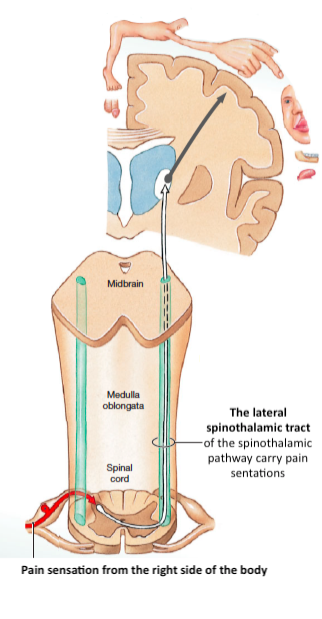
\includegraphics[width=0.5\textwidth]{figures/pathways.png} 
	\caption{Spinothalamic pathway of nociceptor pain. The red arrow indicates the pathway of information from a noxious stimulus. The white arrow indicates the transmission of information towards the brain. The black arrow indicates the pain localization and discrimination in the brain. (Modified \cite{Martini2012})}
	\label{fig:pathways}  
\end{figure}   

%discuss "this part", should it belong to the meditation section? 
%%%Pain is modulated by the descending pathways, where the Periaqueductal Grey (PAG) and the Nucleus Raphe Magnus (NRM) are involved in reducing pain. PAG, also known as anti-nociceptor, is important in the control of pain and surrounds the cerebral aqueduct in Mesencephalon. When this region is electrical stimulated it produces profound analgesia and injection of morphine. PAG receives inputs from the thalamus, hypothalamus, cortex and the spinothalamic tract. Neurons from the PAG region excite the cells in NRM which have a direction towards the spinal cord and block the pain transmission by the dorsal horn cells. Stimulation of NRM produce a strong analgesia and release serotonin which activates the inhibitory interneuron and blocks the pain transmission. The key neurotransmitter is noradrenaline and 5-hydroxytryptamine by modulation pain.~\cite{Steeds2013}
%% stops here ... "this part"


\subsubsection{Neuropathic Pain}
Neuropathic pain is caused by a disorder in the somatosensory system and is often a chronic condition related to injuries or diseases. The disease occurs at different levels in the nervous system and affects the signaling of pain. Compared with nociceptor pain, it is difficult to localize the distribution of neuropathic pain. However, neuropathic pain can be described based on the mechanism and be divided into peripheral, central or mixed syndromes correspond to the anatomy and the underlying disease. This mechanism can produce painful symptoms in the same disease, but it would take different aspects. The sensation can be described as sudden pain which is burning, tingling, shooting, stabbing or numb and can be intermittent or continuous. \cite{Mindruta2013}

%\section{Prevalence of chronic pain}\fxnote{Is this section really necessary?}
%A survey  by \cite{Breivik2006} done in 2006 assessing chronic pain in 15 European countries and Israel found the most common types of chronic pain within 4839 participants suffering from chronic pain. The study found 50 \% of the participants to suffer from back pain, 40 \% suffering from joing pain, especially knee pain and about 20 \% suffering from head pain, neck pain, hand or leg pain. Participants aged between 41-60 suffered mostly from chronic pain. The causes of the pain were mostly due to arthritis, osteoarthritis, traumatic injury and herniated or deteriorating discs within the vertebrae. \cite{Breivik2006}

%% Treatment...

%\begin{table}[H]
%	\begin{tabular}{|l|l|}
% \rowcolor[HTML]{C0C0C0} \rule{0pt}{3ex}  
%	\color[HTML]{000000}{Pain type} & \color[HTML]{000000}{Description} 
% \\ \hline \rule{0pt}{3ex}    
%	 Hyperalgesia &   An abnormal severity of pain followed by a noxious stimulation   
%	\\ \hline \rule{0pt}{3ex}  
%	Hyperpathia &  An exaggerated and prolonged response to stimulation
%	\\ \hline \rule{0pt}{3ex}  
%         Hyperaesthesia &  An increased sensitivity to stimulation.    
%	\\ \hline  \rule{0pt}{3ex} 
%   Dysaesthesia  & \begin{tabular}[c]{@{}l@{}} An evoked or spontaneous altered sensation described \\ as a discomfort rather than pain\end{tabular}
%	\\ \hline  \rule{0pt}{3ex} 
%	  Allodynia &   A painful response to a normally innocuous stimulus.                      
%	\\ \hline
%	\end{tabular}
%	\caption{Pain types divided by the evoked pain~\cite{Steeds2013}.}
%	\label{tab:pain_types}
%\end{table}\vspace{-.25cm}

\section{Assessment of Pain}
Pain is described as a complex and subjective experience that poses a number of measurement challenges due to its subjective nature. Nevertheless, pain measurements are necessary for pain studies as well as the evaluation of methods to control pain.~\cite{Jensen2001} %There is no valid and reliable method of objectively quantifying pain at the moment. 
Despite the challenges that pain measurement present, several tools and approaches can be employed in order to collect useful pain estimates~\cite{Younger2010}. The aim of pain assessment is to diagnose the cause, understand the impact, identify appropriate pain relief strategies and evaluate their effectiveness~\cite{Briggs2010}.

%There are different dimensions of pain experience that can be assessed: intensity, affect, quality and location. Pain intensity defines how much the pain hurts. %, where pain affect is more complex. 
%Pain affect refers the degree of emotional arousal or changes in action due to the sensory experience of pain. Whereas pain quality concerns certain physical perceptions, which are associated with the description of pain, such as pins and needles, prickling or burning. \cite{Jensen2001}

The intensity of pain can be assessed using unidimensional or multidimentional scales ~\cite{Jensen2001}.
 % Changes in pain intensity should only be compared individually and not between subjects, as pain is a subjective experience.
Chronic pain is too complex to assess with unidimensional scales, as the pain affect the patients' functions, quality of life, emotional state, vocational status, social life and well-being, wherefore multidimensional scales are used~\cite{Ebert2010}. 


\subsection{Unidimensional scales}
One used unidimensional scale is the Verbal Rating Scale (VRS), which consists of a list of adjectives describing different levels of pain intensity, as illustrated in \figref{fig:VRS}. This type of scale is easy to administer, score and apprehend. However, it has several statistical disadvantages and criticism raised due to the fact that it assumes equal intervals between the adjectives.~\cite{Jensen2001} For this particular reason along with others, it is only used when the patient's conditions require it~\cite{Jensen1986}. 

\begin{figure}[H]
	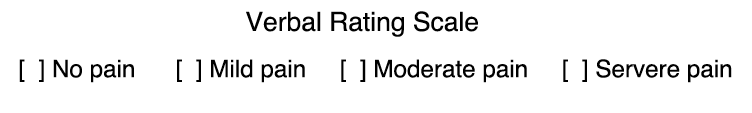
\includegraphics[width=0.5\textwidth]{figures/VRS.png} 
	\caption{Verbal Rating Scale for pain assessment. (Modified \cite{Jensen2001})}
	\label{fig:VRS}  
\end{figure}   

Another possibility of unidimensional scales is a Visual Analogue Scale (VAS). VAS consists of a 10 cm line, as shown in \figref{fig:VAS}. The ends of this line are labeled as the extremes of pain. The scale is scored by measuring the distance from 'no pain' to the patient's mark. This fact makes the VAS more sensitive to changes in pain intensity. However, one of the drawbacks is its evaluation time is higher than for other methods.~\cite{Jensen2001} 

\begin{figure}[H]
	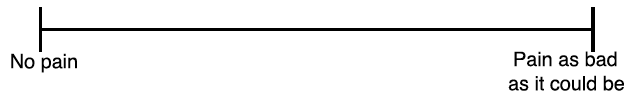
\includegraphics[width=0.5\textwidth]{figures/VAS.png} 
	\caption{Visual analogue scale for pain assessment. (Modified \cite{Jensen2001})}
	\label{fig:VAS}  
\end{figure}   

Another method is the Numerical Rating Scale (NRS), which is illustrated in \figref{fig:NRS}. It is the most used by clinicians, due to the usefulness of administration and scoring. \cite{Fillingim2016} NRS consists of a numerical scale from 0 to 10, describing 0 as 'no pain' and  10 as 'higest level of pain'. The advantage of NRS is that it does not require patients' mobility because the response is given verbally. NRS is a valid method and demonstrates positive and significant correlations with other measurements of pain intensity. \cite{Jensen2001} 

\begin{figure}[H]
	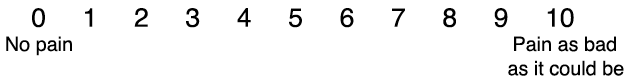
\includegraphics[width=0.5\textwidth]{figures/NRS.png} 
	\caption{Numerical Rating Scale for pain assessment. (Modified \cite{Jensen2001})}
	\label{fig:NRS}  
\end{figure}   

Pictures or face scales can be used to illustrate facial expressions of different intensities of pain. The primary purpose of these scales is to offer individuals with written language or cognitive difficulties, an option to express pain intensity. There is evidence that the pictures or face scales are a valid method. \cite{Jensen2001} 

\subsection{Multidimensional scales}
Multidimensional scales are convenient in relentless pain conditions. There are several  multidimensional scales, whose purpose is to measure several dimensions of pain with different combinations of these dimensions. These scales offer a more detailed reflection of the patient's pain experience than unidimensional scales. \cite{Briggs2010} 

The most frequently used is McGill Pain Questionnaire (MPQ), which consists of 78 words and describes the pain in sensory, affective and evaluative terms. These terms are arranged in groups according to the quality and intensity of pain. A 6-point VRS is used to determine the intensity of the pain. One disadvantage of the MPQ is the length and complexity, wherefore a brief form of this questionnaire has been introduced. The short-form MPQ consists of 15 different descriptors in sensory and affected terms. Each descriptor is rated on a 4-point VRS scale.~\cite{Katz2001}

%Another scale, Brief Pain Inventory (BPI), was developed to assess cancer pain and has been proven as a useful instrument to asses different kinds of pain in several clinical settings. The BPI measures pain severity, pain quality and the disturbance in the patients' daily life. Two subscales score pain intensity and pain interference.~\cite{Katz2001} 

Pain drawing is often used for estimating the location of pain and involves a front and back drawing of the human body. Another used method is the checklist, which is a simple list of possible sites of pain.~\cite{Jensen2001} 


%\subsubsection{Physiological assessment}
%The most commend used for physiological assessment is Back Depression Inventory (BDI), which is used for patients with depression associated to their chronic pain. BDI consist of a questionnaire of 21 question related to the depression. The score of BDI indicated the if the depression is minor, moderate or server. The Spielberger-State-Trait Anxiety Inventory is often used for patient with anxiety beside the chronic pain and consist of 40 item that assess both the stare and trait anxiety.  Furthermore, is the Minnesota Multiphasic Personality Inventory and Coping Strategies Questionnaire. 

\subsection{Quantitative sensory testing}
Quantitative Sensory Testing (QST) is a method to assess the patients' response to quantifiable sensory stimuli in order to characterize the location of pain. QST is used for assessing neuropathic pain and includes different modulations of stimulation, such as thermal, mechanical, electrical, ischemic and chemical. %These stimuli and their intensities can be selected in order to systematically evaluate the somatosensory transmission and pain processing by engaging different nerve fibers, endings and pathways of the central nervous system. 
Approaches for QST used in clinical practice are the Frey monofilaments and tuning forks which are used to measure mechanical sensation. Heated or cooled metal rods can be used to assess thermal sensitivity. The sensitivity of pressure pain can be assessed by an algometer. \cite{Fillingim2016}


\subsubsection{Assessment of Pain Threshold and Tolerance}\label{sec:AoPT}

As a result to a set of experimental noxious stimuli, it is possible to obtain different parameters such as pain threshold or tolerance. 
Psychophysical research has been mostly focusing on threshold measurements. \cite{Pelli2010}
Threshold is defined as the stimulus that produces an arbitrary but defined level of performance. There is a distinction between receptor or absolute threshold and psychophysical or sensory threshold. Absolute threshold is the energy required to elicit response in the primary afferent while the psychophysical or sensory threshold, is the minimal energy necessary to reach perception. Due to the fact that the sensory threshold is higher than the receptor threshold,  the sensory threshold is a convenient parameter which offers the transition point between non-painful and painful stimulus. \cite{Yarnitsky2006} %The pain tolerance is the highest intensity of painful stimulation that a tested subject is able to tolerate. 
%\subsection{Types of psychophysical methods}
The three most common methods used for testing the perception in stimulus detection are the method of adjustment, method of limits and method of constant stimuli.\fxnote{Citation missing}


\begin{itemize}

	\item \textbf{Method of limits}: The magnitude of the stimulus is presented either in ascending or descending order by the examiner. The subject indicates whether or not the stimulus is detected. Accordingly, the threshold in each case is the stimulus magnitude at which the response switches from non-perception to perception and/or vice versa. \cite{Kingdom2016}
	%One of the drawbacks of this method is that the observer may get used to reporting that is perceiving a stimulus or not. As a result, he or she continues to give the same response even at stimulus magnitudes that are higher or lower than the threshold. This phenomena is the error of habituation. Contrarily, the observer may anticipate the response and make a premature judgment, which is call the error of expectation. Another disadvantages using this method is that the parameter value from perception to non-perception differ from non-perception to perception value, due to different artifacts \cite{Hock2010}.
	\item \textbf{Method of adjustment}: This method is a variant of the method of limits, whereby the magnitude of the stimulus is adjusted by the subject until the response switches from non-perception to perception and/or vice versa \cite{Kingdom2016}. %This method is useful for obtaining a rough threshold estimate to guide the choice of stimulus magnitudes for a forced-choice procedure, when there are different conditions to be measured. \cite{Kingdom2016}
	\item \textbf{Method of constant stimuli}: The magnitude of the stimulus is randomly selected from a predefined set. This range is selected to straddle the threshold value. If the data generated by this method fits with the appropriate psychometric function, it provides the most accurate estimates of the threshold. Sometimes the  choice of this stimuli set demands pilot work to obtain an estimate of the threshold. \cite{Kingdom2016}
\end{itemize}

%\section{Symptoms of chronic pain}

%Chronic pain can occur in the whole body. Typical complains of chronic pain patients, regardless of the localization of the pain, is insidious onset of pain, non-localized pain or back pain that radiates to the leg. \cite{marcus2009}

\section{Treatment of chronic pain} \label{sec:treatment}
There are several treatments for chronic pain patients, depending on the modalities and intensity of the pain. Besides conservative methods, alternative methods are applied to reduce chronic pain. %The benefit of the alternative methods is a treatment without the risk of negative side-effects. 
\cite{marcus2009,pope2017}

None of the different treatment methods are enough or sufficient when applied alone. But an individual combination considering the needs of each patient alleviates the suffering of the chronic pain. At the moment it is not possible to cure chronic pain, but to relieve the suffering. \cite{marcus2009,pope2017} 

The commonly used treatment method is medication. The disadvantage of medication is the risk of side effects. In contrast to medication, alternative methods do not provide any negative side effect. However some of those methods require a specialist for instruction and/or application, which results in high cost. \cite{marcus2009,pope2017}
%A lot of different methods for relieving pain exist, some of these will be described in the following subsections. 

\subsection{Medication}
Medication is a common way to treat severe chronic pain patients. %, although there are disadvantages. 
Those medicaments can be divided in three groups, the coanalgesic medicaments, the non-opioid and the opioid analgesics. \cite{marcus2009}

\begin{itemize}
\item \textbf{Coanalgesics} are normally used to treat other diseases, for example depressions, but still provide analgesic qualities. They are often used to treat fibromyalgia, chronic headache and neuropathic pain. Often coanalgesics are combined with analgesicts to extended pain-relief. \cite{marcus2009}

\item \textbf{Non-opioid analgesics} are used to reduce intermittent mild to moderate pain. To this category belong nonsteroidal anti-inflammatory drugs, which decrease inflammation and provide analgesic properties. Non-opioid analgesics are especially used in short-term-therapy. Non-opioid analgesics inhibit the prostaglandin synthesis. Prostaglandin has a protective effect to the organs. A permanent use of non-opioid analgesics encourages prostaglandin effects, which conduct in severe organ toxicity. Known side effects are for example gatrointestinal toxicity, pephrotoxicity and a increased risk of cardiovascular diseases. \cite{marcus2009,stein2007}

\item \textbf{Opioid analgesics} provide stronger analgesic qualities than non-opioid analgesics and show no prostaglandin effect. These analgesics work by bending in the central nervous system to the opioid or NMDA receptors.  Because of this better long-term tolerability, opioid analgesics are used in patients which suffer from chronic non-malignant pain. But the use of opioid analgesics accompanies with the risk of abuse and misuse. Studies have shown that the median time until abusive behavior is 24 months. Treatment targets and specific requirements are set to minimize this risk. \cite{marcus2009,stein2007}
The decision, if non-opioid or opioid analgesics are used, is based on weighing safety, tolerability and effectiveness. The superior effectiveness and the lower organ toxicity of opioid analgesic outweigh the risk of abuse or misuse. \cite{marcus2009} 
\end{itemize}

\subsection{Physical therapy}
Physical therapy is applied with the aim to enhance the patients' flexibility, general fitness and musculature. This is achieved by motion exercises and passive joint mobilization to enhance the muscle function and the joint stability and mobility. A special program is adapted to the patients' needs. Components of this program might be moist heat, cryo therapy, ultrasound and transcutaneous electrical stimulation. Furthermore, assistance can be provided by manual therapy or exercise, which is included to improve the physical fitness, achieve weight loss and decrease the risk of chronic diseases encouraged by inactivity. \cite{marcus2009,pope2017}

\subsection{Lifestyle changes}
Habits or life circumstances can intensify chronic pain. Changes of the lifestyle may help to decrease chronic pain. It is known that the pain sensitivity is negatively enhanced by nicotine. Therefore quit smoking can be a step towards relieving chronic pain.
Furthermore, chronic pain patients often suffer from insomnia. Sleep hygiene should be applied to reduce the occurrences as well as the severity of the sleep disturbances. If insomnia is due to medication, it should be revised, if it is possible to change the medication.
Obesity is a risk factor in the likelihood to  develop chronic pain, this is encouraged by the side effects of obesity like psychological disability or musculoskeletal pain. Besides, it encourages other health problems for example cardiovascular disease or diabetes. To improve this condition, weight loss should be achieved by the combination of diet and exercise. This will influence the recovery abilities from pain positively. \cite{marcus2009,pope2017}

\subsection{Psychological therapy}
%Psychological therapy helps patients to reduce depressions or anxiety and enhance a positive attitude. Also it assists patients to identify necessary lifestyle changes and implement them. \cite{marcus2009,pope2017} 

Psychological therapies have been promoted due to their potential effectiveness for the management of chronic pain and its conequences \cite{Eccleston2002}. Psychological treatments are characterized as cognitive or behavioural strategies \cite{Eccleston2013}which purpose is to helps patients to reduce depressions or anxiety and enhance a positive attitude. Also it assists patients to identify necessary lifestyle changes and implement them. \cite{marcus2009,pope2017}. The most popular treatment program is Cognitive Behavior Therapy (CBT). The patients learn that their chronic pain condition has no cure but can be managed using different skills such as relaxation training, environmental changes or behavoiral experiments \cite{Burger2016}. It has been shown that CBT can reduce pain immediatly after a treatment, however the effect is slight\cite{Eccleston2013}. A limitation of CBT is that issues like psychological trauma, victimization or serious emotional and relational conflict are not addressed.

\subsection{Surgery}
Surgery is a less frequent treatment technique. Commonly it is used to relieve patients from pain due to anatomic abnormalities. \cite{marcus2009,pope2017} In some cases surgery is not a recommended treatment, where risk and benefits of surgery should be considered. In addition to this is surgery also one of the most frequently cases of getting chronic pain, as mention in \autoref{sec:Pain}. Therefore, is should be weighted if it should be harked back to other and less invasive treatment options. \cite{pope2017}

\subsection{Alternative treatments}
Beside the primary treatments others can be considered in a addition to these, also know as alternative treatments. Most of the alternative treatments are often associated with spiritually and is not very well documented, why some people tend to be skeptical for these treatment types. However, many alternative treatments have shown to have an positive effect on chronic pain patients.

\subsubsection{Acupuncture}
Acupuncture is a treatment method where small sterile needles are inserted into the skin of the patient. The needles are inserted at specific acupuncture points related to the type of pain that the patient is experiencing. \cite{Dhanani2011}. Acupuncture has shown promising results in reducing pain in patients with soft tissue around the shoulder joint, headaches, neck and shoulder pain, arthritis/osteoarthritis and low back pain. The effect of acupuncture can last for more than 3 months in 80 \% of the patients \cite{Junnilla1983}. 
%A total of 348 patients where evaluated. The mean reduction of the entire patient group where 68 \%. Showing best results in soft tissue round the shoulder joint, showin a mean reduction of pain by 79 \%. The headache and neck and shoulder patients had a mean reduction by 74 \%. Patients with  arthritis/osteoarthritis showed a mean reduction by 58 \% and the patients with low back pain had a mean reduction by 50 \%. In 80 \% of the patients the effect of the treatment lasted for more than 3 month and 32 \% over one year. \cite{Junnilla1983}
% maybe one of these citeations are to old? 


\subsubsection{Chiropractor}
Chiropractic treatment is adjustment and manipulation of the spine in the patient to alignment the vertebrae of the spine to reduce pressure on the nerves running down the spine \cite{Gerald2013}. In some cases this therapy will after a few treatments, increase flexibility of the spine of the patient and relieve the pain \cite{Peterson2012}.
%In a study by \cite{Peterson2012} evaluating 506 patients with acute and chronic back pain after 3 month of chiropractic treatment.
%Patients undergoing chiropractic treatment showed improvements in their condition and the effect was ongoing after 3 month. \cite{Peterson2012}

\subsubsection{Hypnosis}
%Noxious stimuli increased cerebral blood flow in specific areas of the brain in pain processing,  a the thalamic nuclei anterior cingulate and insular cortices.
Hypnosis is a process where one comes into the state of trance and feels deep relaxation and is open to conversation verbally. Hypnosis is a guided process and can be carried out alone or by others. \cite{Gerald2013} Factors as anxiety, depression and other states of mood and in general the social life of the patient has been shown to play a role in chronic pain. These mechanisms might be altered by hypnosis.
In the literature hypnosis has shown positive results in pain relief, but only on a short term basis. \cite{Dhanani2011}
One of the drawbacks of hypnosis is the lack of standardization in hypnotic induction and interventions \cite{Alkis2010}. Also the hypnosis susceptibility  varies from person to person, why not everyone will have the same effect from it \cite{Spiegel2013}.

\subsubsection{Yoga}
Yoga is a form of mind to body practice discipline, or tradition originating from India. In the practice of yoga different physical postures, breathing techniques and more are the routine. 
Yoga is both, a form of personal evolution, but most popular because of the exercise which benefits the health.
A review by Whitehead et al. \cite{Whitehead2017} found that yoga could improve the functionality of the back and a slight effect of treating pain compared to non-yoga participants. 

\subsubsection{Meditation}
*** Make it more meditation in general - end the section with something about mindfulness *** 

Mindfulness meditation is practicing of being aware in the present moment, a form of mental training. Mindfulness can be practiced through meditation, which is one of the common ways of practicing mindfulness. Mindfulness meditation practice is said to have several health benefits like increase in cognitive function and decrease in stress, depression and anxiety. Through some of these mechanisms pain can be altered, eventually leading in pain relief. \cite{Zeidan2016} 

\section{Mindfulness}
Mindfulness has its roots in Buddhism and yogic tradition and is described as a non-elaborative and non-judgmental awareness of the present moment \cite{Kabat1982,Zeidan2012,Zeidan2016,Tang2017}. Within a mindfulness stage one is focusing from one moment to the other and is aware of emotional, cognitive and sensory events. Those events are perceived as temporary, fading and changeable. Moreover one is neither rating nor reacting cognitive or emotional to those events. The mental state of mindfulness can be achieved by with mental training. \cite{Zeidan2012,Zeidan2016}  Thus can be said that mindfulness meditation is training of the mind \cite{Tang2017}. 

Since thoughts and emotions are involved in the perception of pain, mindfulness provides the ability to relieve pain. Mindfulness cannot cure pain, but the patients will be able to deal with the pain easier and reduce the fear associated with pain. Thereby the patients engage more in their treatment instead of relying and focusing on the effects of medication. \cite{Jacob2016}
Often used methods to reach mindfulness are meditation and yoga practice \cite{Kabat1982}.  In this study meditation was used, because physical limitations are not affecting the meditation practice and no prior knowledge is needed \cite{Tang2017}.


\subsection{Meditation classification}
The most well practiced types of meditation are focused attention (FA) and open monitoring (OM).\cite{Zeidan2016} FA is the training of concentration. The subjects keep their focus at an object or specific thing. Hereby the flow of breath is often used.  If any disturbance comes by, like a thought, sound or other environmental distractions, which will often lead to a drift in attention, the person should always bring the attention back to the focus. \cite{Zeidan2016} OM is the cultivation of open presence. The mind is open to anything, not focusing on any specific thing, just being in the present. If any thought or disturbance comes by, the thought or sensation should be noticed briefly, but then left without thinking more over it. FA is used to slide into OM, therefore it is necessary to master FA before one can reach OM. \cite{ Perlman2016, Zeidan2016,Kabat1982} Hence the chosen meditation practice in this study is FA.


%This kind of meditation has been shown to reduce pain more compared to FA, likely because the areas of the brain affected during this form of meditation is \cite{Perlman2010}

%FA and OM can alter pain in different ways...
%OM is more effective in reducing pain after extensive meditation training compared to FA. \cite{Varilly2012}

%(.....MAYBE WE NEED SOME KIND OF REASONING TO WHY WE CHOOSE TO LOOK INTO MINDFULNESS MEDITATION, LIKE A SUMMARY OF ALL THE METHODS BEFORE GOING INTO MINDFULNESS MEDITATION, AND THEN DIG DEEPER INTO THE FACTS OF MINDFULNESS MEDITATION....)

\subsection{Mechanisms of mindfulness}

Previous research indicates that mindfulness meditation is promising for relieving pain, even though the research is limited, and the mechanisms behind mindfulness meditation are not fully understood yet \cite{Perlman2010}. 
Studies show that enhanced emotion regulation, cognitive control, acceptance and positive mood have been linked with health benefits as well as pain modulation. These mechanisms are modulated during mindfulness meditation practice.

With mindfulness meditation one is able to take the attention away from the emotional component of pain. Therefore meditation practice can reduce the brain process areas related to anticipation of pain, which does not imply that meditation reduce the brain process related with pain. \cite{Brown2010}
Pain as well as meditation alter sensory, cognitive and affective dimensions of subjective experience. Therefore brain areas activated during meditation and nociception should be interconnected in a way. \cite{Zeidan2011}

 A study by Perlman et al. \cite{Perlman2010} shows that practicing meditation could not lower the intensity of pain, but instead lower pain unpleasantness in the participants. \cite{Zeidan2012, Perlman2010} Similarly, a study by Brown and Jones et al. \cite{Brown2010} showed that the greater the experience is with meditation the lower the perception of pain unpleasantness. This results in lower activation of the right inferior parietal cortex (IPC) and midcingulate cortex (MCC).  This findings are supported by a study by Lutz et al. \cite{Lutz2012} which shows that unpleasantness rating of pain decrease with meditation experience.
 

%The typical response, when using a placebo analgesia is increased activation of the dorselateral prefrontal cortex during pain anticipation. This effect predicts reductions in pain perception and activity of pain related brain regions. Mindfulness meditation does not involve dorselateral prefrontal cortex activation. \cite{Zeidan2012}


%The findings on mindfulness meditation and pain modulation are split, but experiments in controlled settings are still needed to confirm, if the effect of mindfulness meditation works on pain modulation. \cite{Zeidan2012, Perlman2010}

%****COMENTS FROM BO*****
A study by Gard et al. \cite{Gard2011} reported that the brain pattern related with pain modulation during mindfulness differs to other pain coping strategies. An increased activation in the rostral anterior cingulate cortex (rACC) and the ventromedial PFC (vmPFC) in the anticipation of pain stage was found for mindfulness practitioners. The activation of this areas has been identify with positive emotions. Furthermore, the study by Gard et al. \cite{Gard2011} found for mindfulness practitioners an increased activation in the rACC/vmPFC while anticipating pain. As well as decreased activation in the bilateral IPFC and increased activation in the posterior insula/S2 when receiving a stimuli. Moreover, a study by Grant et al.\cite{Grant2011} showed that mindfulness practitioners have different neuronal responses to painful stimuli with a greater activation in the insula and thalamus and a decrease activity in PFC.

%\fxnote{....and then we need something like: or maybe a summary of all the methods and then saying, because of this and this, mindfulness meditation will be looked further upon as method for reliving pain...}

%The method of mindfulness meditation will be used for method to relief pain in this project.

%\section{Mindfulness meditation}
%Definition
Different brain regions are involved in the practice of mindfulness meditation. 

\begin{figure}[H]
	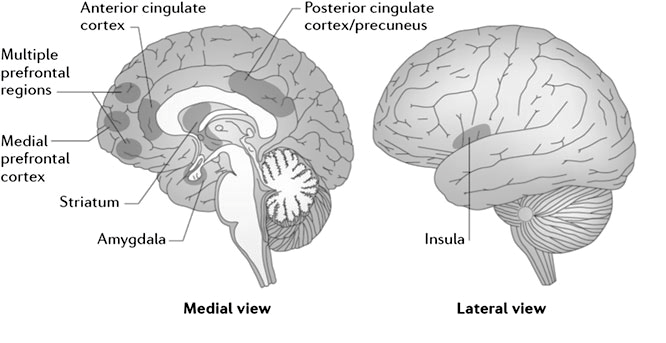
\includegraphics[width=0.9\textwidth]{figures/brain_meditation.png} 
	\caption{Specific regions in the brain involve when practicing mindfulness meditation \cite{Tang2017}.}
	\label{fig:brain_meditation}  
\end{figure}

Hence, the most involved in pain modulation via mindfulness meditation is the PFC and the ACC as illustrated in \figref{fig:brain_meditation}. Furthermore, striatum, insula and Default Mode Network (DMN), which includes the medial PFC and the Posterior Cingulate Cortex (PCC) are shown in \figref{fig:brain_meditation}. These regions play a big role in the effect of mindfulness meditation and are highly regulating the mechanisms of meditation which can generally be catergorized into three catagories: attention control, emotion regulation and self-awareness. 

%Figure \ref{fig:brain_meditation} shows an image of the brain and the regions involved in attention, emotion and self awareness. 
  
\begin{itemize}
	\item \textbf{Attention control} is the ability to maintain focus, for instance on the breath during FA meditation. This mechanism includes mainly ACC, PFC and the striatum, which are illustrated in \figref{fig:brain_meditation} as the red dots. Increased activity in the dorsal lateral PFC is required to hold an increased attention, as well as deactivation of the areas of the brain that makes the mind drift, which include the medial PFC. \cite{Tang2017}
	\item \textbf{Emotion regulation}
	includes the emotions that arise, when they occur and how they are experienced and expressed. This mechanism involves multiple prefrontal regions, limbic regions and striatum, which are regions primary regulating the emotional thoughts through the limbic system also responsible for goal setting. These regions are illustrated as green dots on \figref{fig:brain_meditation}. This need for regulating the emotional control is important because the participant needs to be able to handle boredom or negative mood during the meditation. Stronger subgenual and adjacent ventral ACC activity is present with meditation. This brain area is involved with emotion regulation and attention control. The dorsal lateral PFC and amygdala plays some role in regulation of emotion.  \cite{Tang2017}

	\item \textbf{Self-awareness} includes the awareness of oneself, the awareness of being conscious as well as meta-awareness, which is the awareness of the internal bodily state. Regions of the brain involves midline cortical structure DMN, ACC, the insula, medial PFC and PCC, as illustrated in \figref{fig:brain_meditation} as blue dots. Reduced activity in midline cortical structure including the DMN, more reduction in the posterior part PCC, than the anterior part medial PFC, but increased in perigenual ACC activity.  \cite{Tang2017}
\end{itemize}


\subsection{Stages of meditation}
Different expertises of meditation appear to modulate the dynamic balance between anterior and posterior midline networks involved in different aspects of self, cognitive self, bodily self and phenomenal experiential self. This reflects self plasticity following meditation. 
The effort to get into the meditative state varies according to your experience level with meditation. Often this experience level can be divided into three stages, early, middle and advanced practice of meditation. These stages, illustrated in figure \ref{fig:meditation_stages}, determine the amount of effort to get into the meditative state \cite{Tang2017}. 

\begin{figure}[H]
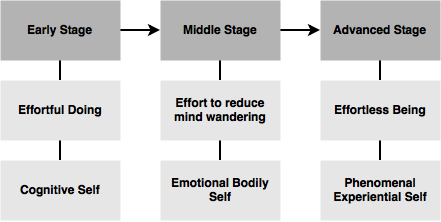
\includegraphics[width=0.8\textwidth]{figures/stages_of_meditation.png} 
	\caption{The three stages of meditation practice describe the effort, which is necessary, to get into the meditative state. \cite{Tang2017}}
	\label{fig:meditation_stages}  
\end{figure}  

In the early stage more mental effort is required. Here the dorsal lateral PFC and partial cortex are often involved and activated more. A stronger deactivation in the DMN occurs when more effort is used. With less effort, the ACC and striatum will participate more. \cite{Tang2017}

The neural mechanisms behind mindfulness meditation in relieving pain has been researched. Experiments with stimulation of nociceptive pain have shown an increase in active areas of the PFC while meditating. Participants express that they feel the pain but are able to deal with it better during meditation focusing on the breath. 
The mechanisms working in analgesia are not the same as the mechanisms during meditation, why the two methods do not interfere with each other. \cite{Jacob2016}

The different areas of the brain show either a reduction or increase in activity when performing meditation. Through meditation the person trains the mind, and specific regions will grow. \cite{Zeidan2012}


%*** Used for state of the art ***
%Examining long term meditators, the findings are a thicker gray matter in mid cingulate cortex and bilateral secondary somatosensory cortex, which are involved in pain related regions overlapping the functional effect. A correlation with the number of years practicing meditaiton and the mid cingulate was also found. This gives evidence to long lasting effects of meditation. \cite{Zeidan2012}
%
%However, short-term mindfulness training can have positive effect in pain relieve. The study by \cite{Zeidan2012} showed an effect of mindfulness meditation practice during four days for 20 min per session, even though most studies conduct the experiments for a period of more than six weeks. \cite{Zeidan2012}

\section{State of the Art} \label{sec:SOTA}
%Chronic pain have been investigated for years in order to understand the mechanism behind. Even though, is it still a relevant issue to explore as many people suffer from chronic pain. Furthermore, is it difficult to treat due to that pain is experienced individually. This also leads to an issue as the assessment of pain is subjective.

%Currently, is there no cure for chronic pain only relieving treatments. The primary treatment is pharmaceutical, which may have side effects, such as toxicity. Alternative treatments, such as therapy, chiropractic and acupuncture have shown to have an impact on relieving pain, but only in a combination with pharmaceutical treatments. The alternative treatments have some disadvantaged due to high costs, why these treatment should be considered.  

%Mindfulness meditation have proved to relieve conditions such as stress, depression and anxiety due to meditations ability to enhance emotion regulation, cognitive control, acceptance and positive mood \cite{Zeidan2012, Zeidan2016}. Studies have also investigated the usefulness of mindfulness meditation for people with chronic pain with similar results.

%Previous studies… 

Chronic pain has been investigated for years in order to understand the mechanisms behind and the topic is still relevant to explore as many people suffer from chronic pain. Furthermore, it is an issue that pain is difficult to treat due to the individually experience of pain and the subjective assessment of pain. \cite{Briggs2010,Norton1999}

Currently there is no cure for chronic pain, only relief treatments. The primary treatment is pharmaceutical, which has possible side effects, such as abuse or toxicity. Alternative treatments like physical therapy, chiropractic and acupuncture have shown an impact in relieving pain. But these treatments will most likely be used in combination with pharmaceutical treatments. Many alternative treatments have disadvantages such as high costs, why the decision for these treatments should be considered well, to ensure that it suits the patients’ needs and to maximise the effect for the cost. \cite{marcus2009,pope2017}

Mindfulness meditation has proved to relieve conditions such as stress, depression and anxiety through the ability to enhance emotion regulation, cognitive control, acceptance and positive mood \cite{Zeidan2012,Zeidan2016}. Studies have investigated the usefulness of mindfulness meditation for people with chronic pain showing promising results in pain relief. \cite{Kabat1982,Rosenzweig2010}

%Mindfulness meditation was conceived in the late 1970s and spotted for patients suffering from chronic pain \cite{Chiesa2010}. There is ambiguity within the literature due to the different meditative practices under the term 'mindfulness'. Different studies divide this technique in two styles FA and OM \cite{Lutz2008,Zeidan2012}. Some surveys presented that particularly OM practice is associated with pain reduction \cite{Grant2009,Perlman2010}. 
% **** ADD something about FA - that it maybe easier?? **

The most commonly used mindfulness-based intervention is Mindfulness Based Stress Reduction (MBSR) \cite{Cramer2012}. MBSR consist of 8 or 10 weeks of mindfulness meditation where the patient have to attend once a week a course for 2 hours and 45 minutes session at home 6 days per week \cite{Kabat1982, Chiesa2010}. Patients suffering from chronic pain improved pain symptoms as well as life quality after the finalization of MBSR \cite{Zeidan2012}.
%An extent of MBSR is Cognitive Behavioral Therapy (CBT)\fxnote{Check CBT!}, which incorporates elements of cognitive therapy facilitating a detached view of one's thoughts and is designed to prevent depressive relapse \cite{Chiesa2010}. 
Patients suffering from chronic pain improved pain symptoms as well as life quality after the finalization of MBSR. \cite{Zeidan2012} 
%
%However, studies showed no difference using MBSR or CBT to relieve chronic pain, as both illustrated positive effect compared with usual care \cite{Jacob2016,Cherkin2016}. 
Hence, MBSR provides significant improvement for patients suffering from neck pain \cite{Rosenzweig2010}.

Even though long-term mindfulness meditation is the most investigated, short-term mindfulness training has also shown relief of pain. The studies have investigated different duration of meditation practice and time period within short-term mindfulness meditation. Consequently the boundaries of short-term mindfulness meditation are not well defined. A study by Ussher et.al. \cite{Ussher2012} showed in a clinical setting that 10 minutes mindfulness-based body scan reduces distress and the perception of pains’ impact on daily living. However, the study found no effect outside the clinical environment \cite{Ussher2012}. Another study by Zeidan et.al. \cite{Zeidan2012} proved that only three days of mindfulness meditation with a 20 minutes session each day have an effect on relieving chronic pain. 

Some studies have studied the effect of mindfulness meditation for musculoskeletal chronic pain unifying lower and upper back pain, shoulder and cervical pain \cite{Chiesa2010}. Nevertheless, there is not much literature available focusing on chronic neck pain, which about 25 \% of the patients suffer from \cite{Macfarlanea2016}. The most investigated method is MBSR, mostly over a time period of two months or more. A shorter time period of mindfulness meditation has not been investigated focusing on neck pain.



\chapter{Problem formulation}
%Approximately 375 million people suffer from chronic neck pain. The primary treatment for those patients is medication. But medication has side effects, as described in \ref{sec:treatment}.  Besides medication, alternative treatment methods are used, often in combination with medication. For example physical therapy, chiropractor or psychological therapy have showed a positive influence on pain relief. Most of the alternative treatment methods are related with high costs, because they require a specialist for the application. Whereas mindfulness meditation can be practiced alone. Hence a lot of studies focused on the ability of mindfulness meditation to relieve pain.
%As mentioned in \ref{sec:SOTA}, there are not many studies which show the effect of mindfulness meditation on chronic neck pain. Since a lot of people suffer from chronic neck pain this study investigates the influence of mindfulness meditation on neck pain. 

Pain levels of chronic pain patients are difficult to assess and quantify. Chronic pain patients experience a habituation effect to the pain. Additionally there are variations of the pain sensitivity between days and throughout the day which makes it difficult to get reliable and comparable pain levels of these patients. Since chronic pain is a subjective and multidimensional experience, another way to get comparable values of pain was chosen. Therefore pressure pain was applied with an algometer on healthy subjects. The application of pressure with an algometer was chosen to assess pain, because pressure satisfies the requirements of an suitable method for the quantification of pain \cite{Keele1954}. Hence pressure pain threshold (Threshold) and pressure pain tolerance (Tolerance) values were used to test the following hypothesis:
%\textit{Short-term mindfulness meditation practice increases the pressure pain threshold and the pressure pain tolerance in the upper trapezius.}
\textit{Short-term mindfulness focused attention meditation practice on 5 consecutive days increases the pressure pain threshold and pressure pain tolerance in the right upper trapezius}. In this study meditation was used, because physical limitations are not affecting the meditation practice and no prior knowledge is needed \cite{Tang2017}. In mindfulness meditation FA is used to slide into OM, therefore it is necessary to master FA before one can reach OM \cite{Perlman2016, Zeidan2016,Kabat1982}. Hence the chosen meditation technique in this study is FA. The upper trapezius was chosen for the pressure application, because it is involved in chronic neck pain and has the lowest Threshold values compared with other muscles \cite{Falla2004,Fischer1987}. Even though the study was conducted in healthy subjects, the sensation of the pain and the effects of meditation to the pain sensitivity can be transferred to chronic pain patients \cite{Kjogx2016}.






\chapter{Methods}
%\section{Protocol} \fxnote{Did we want to add something about asking them about the pain after each methods? or what did we discuss about this}
%This protocol will describe the present study, which consist of two experiments testing pain tolerance and pain threshold after practicing mindfulness meditation or after not practicing mindfulness meditation. 

%\section{Purpose}
%The treatment of chronic pain has constraints, as the treatments are only relieving the pain instead of curing the pain. Another issue is that some of these treatments, example medication, have side effect, as described in \secref{sec:treatment}. 
%There is alternative to medication such as yoga, hypnosis and physical therapy, psychological therapy and chiropractor, which have shown to have an influence on relieving pain. But these treatments are often used in combination with pharmaceutical treatment. Furthermore, most of these alternative require an external person to apply, which can result in high costs, as mention in \secref{sec:treatment}.
%An alternative to the present treatment is mindfulness meditation, which have shown an effect on relieving conditions as stress, depression and  anxiety through the ability to enhance emotion regulation, cognitive control, acceptance and positive mood, as described in \secref{sec:SOTA}. 
%Different studies have shown that practicing meditation have an effect on reliving pain. However, these studies have most often investigated long-term mindfulness meditation for patient with eater chronic pain or low back pain. There is a limit on studies that have investigated short-term in patient with neck pain, why this could be interesting to investigate further, as approximately 25\% of the chronic pain patients suffer from this condition. In order to investigated the influence of mindfulness meditation on pain threshold and pain tolerance for people with neck pain following hypothesis is proposed:

%Approximately 375 million people suffer from chronic neck pain. The primary treatment for those patients is medication. But medication has side effects, as described in \secref{sec:treatment}.  Besides medication, alternative treatment methods are used, often in combination with medication. For example physical therapy, chiropractor or psychological therapy showed a positive influence on pain relief. Most of the alternative treatment methods are related with high costs, because they require a specialist for the application. Whereas mindfulness meditation can be practiced alone. Hence a lot of studies focused on the ability of mindfulness meditation to relieve pain.
%As mentioned in \secref{sec:SOTA}, there are not many studies which show the effect of mindfulness meditation on chronic neck pain. Since a lot of people suffer from chronic neck pain this study investigates the influence of mindfulness meditation on neck pain. %Pain levels of chronic pain patients are not very easy to access and to quantify, therefore pressure pain was applied with an algometer on healthy subjects, 

%Pain levels of chronic pain patients are not very easy to access and to quantify because the pain is neuropathic and the assessment is multidimensional and the experience of pain is subjective. Therefore, in order to get some quantifiable measures on pain to clarify if mindfulness meditation will have an effect on sensitivity of pain, acute pain in the form of pressure pain was applied to healthy subjects. If the pressure pain tolerance is increased, after practicing mindfulness meditation, in the upper trapezius it might also have an effect on pain in other body parts. And if it is possible to show an effect on acute pain due to an increase in the tolerance on healthy subjects it might also be possible to help relieving pain in chronic pain patients. On basis of this the study wants to test the following hypothesis:

%***** This part should be more convincing ****
%Pain levels of chronic pain patients are not very easy to access and to quantify because the assessment of neuropathic pain is multidimensional and the experience of chronic pain is subjective. Also variation of the patients' pain from day to day and throughout the day makes it difficult to get reliable and comparable  values of the pain levels of these patients. Therefore acute pressure pain was applied with an algometer to healthy subjects to get quantifiable values of pain and test the following hypothesis: 
%*** Until here ***


%\textit{Short-term mindfulness meditation practice increases the pressure pain threshold and the pressure pain tolerance in the upper trapezius.}

%\vspace{-.5cm}
%\begin{itemize}
%\item Short-term mindfulness meditation increases the pressure pain threshold and the pressure pain tolerance.
%\end{itemize}

\section{Subjects}
%Forty healthy subjects were recruited for the experiment, 20 males (M) and 20 females (F) with a mean age $\pm$XX. A homogeneous group of participants were enrolled in order to limit the amount of variables in the study. For insuring this, specific inclusion and exclusion criteria have been formed for this experiment. 
42 healthy subjects were recruited for the experiment, 21 males (M) and 21 females (F) with a mean age of 23.93 $\pm$ 2.74 years. To get a homogeneous group of participants, specific inclusion and exclusion criteria were  formed for this experiment.

\textbf{Inclusion criteria:}
\vspace{-.5cm}
\begin{itemize}
	%\item Healthy
	\vspace{-.3cm}
	\item Age between 20 and 30 years
	\vspace{-.3cm}
	\item No obesity
	\vspace{-.3cm}
	\item Must have time to meditate for 5 days, 20 minutes per day.
\end{itemize}

\textbf{Exclusion criteria:}
\vspace{-.5cm}
\begin{itemize}
	\item Ongoing meditation practice 
	\vspace{-.3cm}
	\item Pregnancy 
	\vspace{-.3cm}
	\item Neurological, musculoskeletal or mental illness
	\vspace{-.3cm}
	\item Abusive drug or alcohol use \fxnote{Think about this 'abusive'}
		\vspace{-.3cm}
			\item Medication with antidepressant or analgesic properties
\vspace{-.3cm}
	\item Lack of ability to cooperate
\end{itemize}

\vspace{-.5cm}
%Furthermore, is it not necessary that subjects believe in the effect of mindfulness meditation.\fxnote{I don't know about this sentence, i think it does not fit in here. Maybe it is more something we should write for the participants or could we put it in as one of our criteria?.}

\section{Study design} 
%For this particular experiment a parallel study was conducted. The subjects recruited for the experiment were randomly assigned in two different groups, the control group or the treatment group, with a equal amount of female and males in the groups. The control group consisted of twenty subjects no meditation. The treatment group consisted of twenty subjects meditation. The structure of the study design is illustrated on \figref{fig:studydesign}. 
%For this particular experiment a random controlled study was conducted. 

The subjects, recruited for the experiment, were assigned in two different groups. Whereby an equal amount of females and males were assigned. The treatment group was measured before and after the intervention, which was the practice of mindfulness meditation. To ensure that a measured effect was not due to habituation to the measurement, a control group was measured with the same time difference. Moreover, to minimize bias, the examiner was blinded. The structure of the study design is illustrated on \figref{fig:studydesign}.

\begin{figure}[H]
	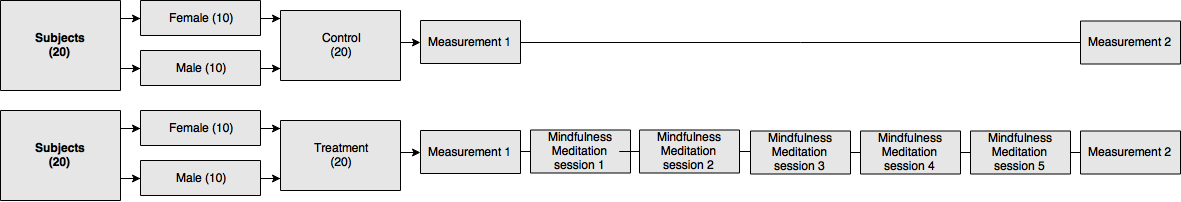
\includegraphics[width=1\textwidth]{figures/studydesign.png} 
	\caption{Parallel study design.}
	\label{fig:studydesign}  
\end{figure}  

%There will be seven to eight days between the measurements. The treatments groups start practicing mindfulness meditation three or four days after the first measurement and will then practice mindfulness meditation for five days and will on the last day of meditation be measured again.

%\section{Setup}
%The Pressure Pain Threshold (PPT), defined as the pressure at which the sensation changed from pressure to pain, has been recognized as an effective and reliable way to quantify pain measures. In this study PPT was measured using Wagner Force Ten$^{TM}$ Digital force Gage. PPT were measured in the upper trapezius. Testing points were marked to ensure reliable and rapid location during the experimental procedure. 
%The algometer was applied four times, two on the left side and two on the right side of the upper trapezius, and the average of the registrations was filed. The subjects had a 5 minutes resting time between measurements. PPT values were measured two times, the first day of the study and after 5 days since the first measure.

%\subsubsection{Mindfulness meditation}
%The treatment group should do guided meditation for 30 minutes in small groups for 5 days. On the first day the mediators would be giving a short introduction to mindfulness meditation. During the meditation the subjects would be in a sitting position with the face  away from the other subjects, to assure that they would not get distracted. 


\section{Procedure}
First of all, general information about the subjects’ were collected, such as gender and BMI, which is illustrated in  \tabref{tab:subjectsA} and \tabref{tab:subjectsB} in Appendix \ref{SubjectINFO}. Furthermore, information about the experiment was given to the subjects. Measurement points were marked at the upper trapezius on right side, as illustrated on \figref{fig:trapezius} while the subjects lay prone to ensure reliable and rapid location during the experimental procedure. The location of the upper trapezius was determined between the acromion and 7th cervical vertebra. The distance was notated so the same locations could be used for each measurement session. 

\begin{figure}[H]
	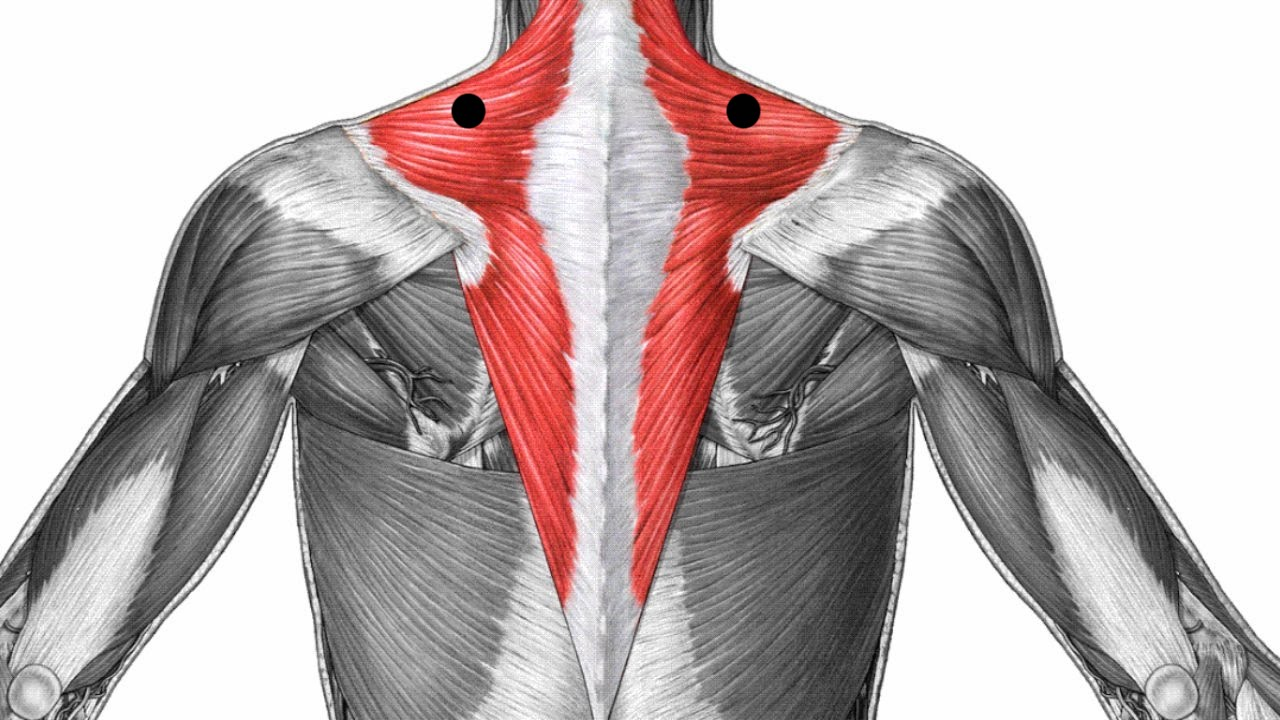
\includegraphics[width=0.5\textwidth]{figures/trapezius} 
	\caption{Measurement on the upper trapezius. The measurement points are mark with black dots.}
	\label{fig:trapezius}  
\end{figure}  

The pressure pain threshold was measured with an algometer (Wagner Force Ten ™  Digital force Gage). Firstly, the algometer was applied until the subject begins to feel pain and the pain threshold was notated. Secondly, the pressure pain tolerance was measured with the same algometer at the same points and the pressure was applied until the subject reached the maximum level of pain.

The same measurement routine was conducted three times. Each measurement was notated and an average was used for the pain threshold and pain tolerance respectively. To avoid oversensation, there was 5 minutes pause in between the measurements. 

To test the effect of mindfulness meditation on the pressure pain threshold and the pressure pain tolerance, the treatment group practiced 20 minutes mindfulness meditation for 5 consecutive days. To ensure same meditation conditions for all of the subjects, a guided meditation in form of an audio file was used. Furthermore, subjects were told to have the most comfortable position during the meditation.  Additionally a short introduction to mindfulness meditation was provided on the first day. 

The subjects of the control group continued their normal routine.
After the last meditation session of the treatment group the second measurements were conducted. The same time interval between the measurements were used for the subjects of the control group. The second measurement session was conducted likewise the first measurements.


\section{Data Analysis}
First the Shapiro-Wilk test was applied to evaluate the normality of the samples. Thereby the sample scores are compared with the scores, which are anticipated under normal distribution.The Shapiro-Wilk test has shown to be valid even in small samples (n < 20), wherefore it was chosen for this study. \cite{Shapiro1965,Mooi2018}


According to the outcome of the Shapiro-Wilk test either a non-parametric or a parametric test was chosen.
For comparison of treatment and control group with regards to threshold and tolerance of first and second measurement a Kruskal-Wallis test was applied in the case of a non-parametric distribution and a two-way mixed ANOVA was applied in the case of a normal distribution.
For comparison of treatment and control group with regards to the difference in threshold and tolerance as a percentage of first and second measurement a Mann-Whitney-U test was applied in the case of a non-parametric distribution and a t-test was applied in the case of a normal distribution.




\chapter{Data analysis}

\chapter{Results}
\section{Subject information}

** WRITE SOMETHING HERE ***

\subsection{Subject information - Control}
\begin{longtable}{l|c|c|c|c|c}
	\rowcolor[HTML]{C0C0C0} \rule{0pt}{3ex}  \color[HTML]{000000}{Gender} & \color[HTML]{000000}{Age} & \color[HTML]{000000}{Weight} & \color[HTML]{000000}{Height} &  \color[HTML]{000000}{BMI} 
	\\ \hline \rule{0pt}{3ex} 
	F(12) M(10) & $\pm$ & $\pm$  &  $\pm$ &  $\pm$ 
	\\ \hline 
	\caption{Distribution of subjects for the treatment group. Gender is indicated with either F (female) or M (male). The means and standard deviations are calculated for age, height, weight and BMI.}
	\label{tab:subjects}
\end{longtable}
\vspace{-.5cm}


\subsection{Subject information - Treatment}
\begin{longtable}{l|c|c|c|c|c}
	\rowcolor[HTML]{C0C0C0} \rule{0pt}{3ex}  \color[HTML]{000000}{Gender} & \color[HTML]{000000}{Age} & \color[HTML]{000000}{Weight} & \color[HTML]{000000}{Height} &  \color[HTML]{000000}{BMI} 
	\\ \hline \rule{0pt}{3ex} 
	F(12) M(10) & $\pm$ & $\pm$  &  $\pm$ &  $\pm$ 
	\\ \hline 
	\caption{Distribution of subjects for the control group. Gender is indicated with either F (female) or M (male). The means and standard deviations are calculated for age, height, weight and BMI.}
	\label{tab:subjects}
\end{longtable}
\vspace{-.5cm}

\chapter{Discussion}

\chapter{Conclusion}

\urlstyle{same}
\printbibliography

\chapter{Appendices}
\section{Subject information - Treatment}
\begin{longtable}{l|c|c|c}
	\rowcolor[HTML]{C0C0C0} \rule{0pt}{3ex}  \color[HTML]{000000}{Subject} & \color[HTML]{000000}{Gender} & \color[HTML]{000000}{Age} &  \color[HTML]{000000}{BMI} 
	\\ \hline \rule{0pt}{3ex} 
\#T1 & F  & 25  & 27.44  \\ \hline \hline \rule{0pt}{3ex} 
\#T2 & F & 23 & 23.14  \\ \hline \hline \rule{0pt}{3ex} 
\#T3 & M & 22 & 21.13  \\ \hline \hline \rule{0pt}{3ex} 
\#T4 & F & 21  & 22.68  \\ \hline \hline \rule{0pt}{3ex} 
\#T5 & F & 22 & 21.58   \\ \hline \hline \rule{0pt}{3ex} 
\#T6 & F & 20 & 23.12 \\ \hline \hline \rule{0pt}{3ex} 
\#T7 & M & 25  & 25.06  \\ \hline \hline \rule{0pt}{3ex} 
	\#T8 & F & 21 & 24.96  \\ \hline \hline \rule{0pt}{3ex} 
	\#T9 & F & 22 & 21.38   \\ \hline \hline \rule{0pt}{3ex} 
	\#T10 & F & 34 & 24.28  \\ \hline \hline \rule{0pt}{3ex} 
	\#T11 & F & 21 & 21.13 \\ \hline \hline \rule{0pt}{3ex} 
\#T12 & M  & 24  & 26.23\\ \hline \hline \rule{0pt}{3ex} 
\#T13 &  F & 25 & 19.27 \\ \hline \hline \rule{0pt}{3ex} 
\#T14 & M  & 22 & 20.76  \\ \hline \hline \rule{0pt}{3ex} 
\#T15 & M & 23 & 28.07  \\ \hline \hline \rule{0pt}{3ex} 
\#T16 & M & 24 & 31.10 \\ \hline \hline \rule{0pt}{3ex} 
\#T17 & M & 23 & 24.49  \\ \hline \hline \rule{0pt}{3ex} 
	\#T18 & M & 22 & 21.16 \\ \hline \hline \rule{0pt}{3ex} 
	\#T19 & M & 27 & 25.17 \\ \hline \hline \rule{0pt}{3ex} 
	\#T20 & M & 23  & 23.21  \\ \hline \hline \rule{0pt}{3ex}
		\#T21 & M & 26 & 26.64   \\ \hline \hline \rule{0pt}{3ex} 
	%\rowcolor[HTML]{C0C0C0} \rule{0pt}{3ex} \color[HTML]{000000}{Mean{\color[HTML]{C0C0C0}X}} 
	Mean & F(10) M(11) & 23.57 $\pm$ 2.99  & 23.90 $\pm$ 2.90
	\\ \hline 
	\caption{Subject characteristics. Gender is indicated with either F (female) or M (male). The means and standard deviations are calculated for age and BMI.}
	\label{tab:subjects}
\end{longtable}
\vspace{-.5cm}


\section{Subject information - Control}
\begin{longtable}{l|c|c|c}
	\rowcolor[HTML]{C0C0C0} \rule{0pt}{3ex}  \color[HTML]{000000}{Subject} & \color[HTML]{000000}{Gender} & \color[HTML]{000000}{Age}  &  \color[HTML]{000000}{BMI} 
	\\ \hline \rule{0pt}{3ex} 
\#C1 &  F & 23 & 21.89 \\ \hline \hline \rule{0pt}{3ex} 
\#C2 & F & 25 & 23.84 \\ \hline \hline \rule{0pt}{3ex} 
\#C3 & F & 27 & 21.13 \\ \hline \hline \rule{0pt}{3ex} 
\#C4 & F & 27 & 20.96\\ \hline \hline \rule{0pt}{3ex} 
\#C5 & M & 24 & 28.06 \\ \hline \hline \rule{0pt}{3ex} 
\#C6 & M & 23 &  24.74 \\ \hline \hline \rule{0pt}{3ex} 
\#C7 & F & 22 & 23.77 \\ \hline \hline \rule{0pt}{3ex} 
	\#C8 & M & 24 & 21.91 \\ \hline \hline \rule{0pt}{3ex} 
	\#C9 & M & 22 & 27.17  \\ \hline \hline \rule{0pt}{3ex} 
	\#C10 & M & 23 &  22.59 \\ \hline \hline \rule{0pt}{3ex} 
\#C11 & F & 23  & 21.30 \\ \hline \hline \rule{0pt}{3ex} 
\#C12 & M & 27 & 22.74 \\ \hline \hline \rule{0pt}{3ex} 
\#C13 & F  & 21 & 32.80  \\ \hline \hline \rule{0pt}{3ex} 
\#C14 & M &  23 & 20.28 \\ \hline \hline \rule{0pt}{3ex} 
\#C15 & F & 24 &  20.28 \\ \hline \hline \rule{0pt}{3ex} 
	\#C16 & F & 22  & 20.28 \\ \hline \hline \rule{0pt}{3ex} 
	\#C17 & F  & 22 &  21.37\\ \hline \hline \rule{0pt}{3ex} 
	\#C18 & F & 23  & 18.17   \\ \hline \hline \rule{0pt}{3ex}
		\#C19 &  M & 29 & 31.21 \\ \hline \hline \rule{0pt}{3ex} 
	\#C20 & M & 26 & 26.58  \\ \hline \hline \rule{0pt}{3ex}  	
	\#C21 & M & 30 & 21.80  \\ \hline \hline \rule{0pt}{3ex}  
Mean & F(10) M(11) & 24.29 $\pm$ 2.47 & 23.43 $\pm$ 3.67
	\\ \hline 	
	\caption{Subject characteristics. Gender is indicated with either F (female) or M (male). The means and standard deviations are calculated for age and BMI.}
	\label{tab:subjects}
\end{longtable}
\vspace{-.5cm}


\begin{appendices}

\end{appendices}

\end{document}
